\documentclass[9pt,conference]{IEEEtran}
\IEEEoverridecommandlockouts
% The preceding line is only needed to identify funding in the first footnote. If that is unneeded, please comment it out.
\usepackage{cite}
\usepackage{amsmath,amssymb,amsfonts}
\usepackage{algorithmic}
\usepackage{graphicx}
\usepackage{textcomp}
\usepackage{xcolor}
\def\BibTeX{{\rm B\kern-.05em{\sc i\kern-.025em b}\kern-.08em
    T\kern-.1667em\lower.7ex\hbox{E}\kern-.125emX}}


% Our packages
\usepackage{booktabs}
\usepackage{subcaption}
\usepackage{soul}
\usepackage{url}

\usepackage{tabularx}
\newcolumntype{P}{>{\raggedright\arraybackslash}X}
\newcolumntype{C}{>{\hsize=0.5\hsize}X}
\usepackage{makecell}
\usepackage{multirow}
\usepackage{pifont}% http://ctan.org/pkg/pifont

% Custom commands
\newcommand{\cmark}{\ding{51}}%
\newcommand{\xmark}{\ding{55}}%

\newcommand*\circled[1]{\tikz[baseline=(char.base)]{
            \node[shape=circle,draw,inner sep=0.75pt] (char) {\small #1};}}

\newcommand{\comment}[1]{{\color{red} [{#1}]}}          % shortcut for visible remark
\newcommand{\fixme}[1]{{\color{red} {#1}}}          % shortcut for visible remark

\newcommand{\sophia}[1]{{\color{red} Sophia: [{#1}]}}

\begin{document}
\bstctlcite{IEEEexample:BSTcontrol}

\title{Gemmini: Enabling Systematic Deep-Learning Architecture Evaluation via Full-Stack Integration}

% \author{Hasan Genc (\texttt{hngenc@berkeley.edu}), Seah Kim, Alon Amid, Ameer Haj-Ali, Vighnesh Iyer, Pranav Prakash, Jerry Zhao, \\
% Daniel Grubb, Harrison Liew, Howard Mao, Albert Ou, Colin Schmidt, Samuel Steffl, John Wright, \\
% Ion Stoica, Jonathan Ragan-Kelley, Krste Asanovic, Borivoje Nikolic, Yakun Sophia Shao \\
% UC Berkeley}

% \author{\IEEEauthorblockN{1\textsuperscript{st} Author}
% \IEEEauthorblockA{\textit{1\textsuperscript{st} Institution} \\
% email1@example.edu}
% \and
% \IEEEauthorblockN{2\textsuperscript{nd} Author}
% \IEEEauthorblockA{\textit{2\textsuperscript{nd} Institution} \\
% email2@example.edu}
% }

\author{\IEEEauthorblockN{Hasan Genc*, Seah Kim*, Alon Amid*, Ameer Haj-Ali*, Vighnesh Iyer*, Pranav Prakash*, Jerry Zhao*, Daniel Grubb*,\\ Harrison Liew*, Howard Mao*, Albert Ou*, Colin Schmidt*, Samuel Steffl*, John Wright*, Ion Stoica*,\\ Jonathan Ragan-Kelley†, Krste Asanovic*, Borivoje Nikolic*, Yakun Sophia Shao*}
\IEEEauthorblockA{\textit{*UC Berkeley, †MIT} \\
hngenc@berkeley.edu}
\vspace{-0.25in}
}

\maketitle

%%%%%% -- PAPER CONTENT STARTS-- %%%%%%%%

%% \section{Organization}

\textbf{Main idea of paper:} full-stack integration (programming model, SoC, RTL, etc.) is needed to accurately investigate accelerator performance/efficiency

\textbf{Sections:}
\begin{itemize}
    \item Abstract and Introduction: 0.75 page
    \item Background and Motivation: 1 page
        \begin{itemize}
            \item I would really like to keep the table if possible
        \end{itemize}
    \item Gemmini Design: 1.25 pages
        \begin{itemize}
            \item \textit{Architectural template:} 0.5 pages
            \item \textit{Programming support:} 0.5 pages
            \item \textit{System parameters:} 0.5 pages
            \item This will require some rewriting, because the focus will be on the full-stack integration, rather than the paramterizability
            \item Make clear that we have convolution, and talk about how we support it without im2col data duplication. Also mention that we have pooling, transpose, etc., but don't spend entire paragraphs on it.
            \item Spend one paragraph introducing programming modes and one paragraph talking about data-staging, and one paragraph introducing virtual memory.
        \end{itemize}
    \item Evaluation: 1 page
        \begin{itemize}
            \item If we can't get to NVDLA-like performance one week before the deadline, 
            then remove the NVDLA comparison.
            \item DAC papers usually have detailed evaluation metrics. Keep the tables, but cut down on text here. (E.g. cut down on paragraph that talks about P\&R stats, but keep the table).
        \end{itemize}
    \item Case Study: Virtual Memory: 0.75 pages
        \begin{itemize}
            \item Should we reword this to make the language less assertive?
            \item Try to frame this as a co-design ``problem'' instead of a characterization
            \item Show how much the single-register reduces burstiness of requests
        \end{itemize}
    \item Case Study: Scratchpad vs L2: 1 pages
        \begin{itemize}
            \item Frame this more clearly as a memory partitioning and codesign problem, rather than a resource contention characterization.
        \end{itemize}
    \item Conclusion: 0.25 pages
\end{itemize}

\hl{Highlighted text} should be removed. \textcolor{red}{Red text} are notes.
\newpage



\begin{abstract}

DNN accelerators are often developed and evaluated in isolation without considering the cross-stack, system-level effects in real-world environments. This makes it difficult to appreciate the impact of System-on-Chip (SoC) resource contention, OS overheads, and programming-stack inefficiencies on overall performance/energy-efficiency. To address this challenge, we present Gemmini, an open-source\footnote{\url{https://github.com/ucb-bar/gemmini}},
full-stack DNN accelerator generator. Gemmini generates a wide design-space of efficient ASIC accelerators from a flexible architectural template, together with flexible programming stacks and full SoCs with shared resources that capture system-level effects. Gemmini-generated accelerators have also been fabricated, delivering up to three orders-of-magnitude speedups over high-performance CPUs on various DNN benchmarks. % Gemmini is open-sourced at \url{https://github.com/ucb-bar/gemmini}.

\end{abstract}

%=============Full, 200-word abstract below==============
% Rapid advances in Deep Neural Networks (DNNs) have resulted in high demand for efficient DNN hardware accelerators.
% However, DNN accelerators are often developed and evaluated in isolation without considering the cross-stack, system-level effects in real-world execution environments.
% This makes it difficult for researchers and engineers to appreciate the impact of System-on-Chip (SoC) resource contention, OS overheads, and programming-stack inefficiencies on overall performance and energy efficiency.
% To address this challenge, we present Gemmini, a full-stack, open-source DNN accelerator generator that enables systematic evaluations of deep-learning architectures.
% Gemmini generates a wide design-space of efficient DNN ASIC accelerators based on a flexible architectural template, together with a full SoC execution environment with host CPUs and shared resources to capture system-level effects.
% Gemmini also provides a multi-level software flow that allows researchers to investigate the impacts of both high- and low-level programming models on DNN performance and programmer productivity.
% % Gemmini results
% Gemmini-generated DNN accelerators have been successfully fabricated, and they can deliver up to 2,670x speedup with respect to a baseline CPU across a range of DNN benchmarks, and comparable speedup to state-of-the-art, commercial DNN accelerators. We also demonstrate, through several case studies, how Gemmini enables hardware designers to understand system-level behaviors for emerging DNN applications.




%==================OLD TEXT BELOW=============================
%A large majority of DNN accelerators, however, target a single hardware design
%point to accelerate the main computational kernels of deep neural networks. %
%such as convolutions or matrix multiplication.
%On the other hand, the spectrum of use-cases for neural network accelerators,
%ranging from edge devices to cloud, presents a prime opportunity for agile
%hardware design and generator methodologies.

% Gemmini runs with the RISC-V ISA, and is integrated with the Rocket Chip System-on-Chip generator ecosystem, including Rocket in-order cores and BOOM out-of-order cores.

%\textcolor{red}{Through several case studies, we show that Gemmini excels at
%system-level integration, and hardware configurability. We also support multiple
%frontends, allowing architects and programmers to choose between multiple
%programming models, which each make different tradeoffs between fixed hardware
%costs, runtime performance, and developer productivity.}
%Gemmini-generated accelerators were used in the fabrication of test
%systems-on-chip in TSMC 16nm and Intel 22FFL process technologies, achieving
%\textcolor{red}{comparable performance to NVDLA}.

\section{Introduction}

% \textcolor{red}{Start from applications, rather than from high-productivity hardware design. Just one sentence should be enough.}
Deep neural networks (DNNs) have gained major interest in recent years in application domains ranging from computer vision, to machine translation, to robotic manipulation.
However, running modern, accurate DNNs with high performance and low energy consumption is often challenging without dedicated accelerators which are difficult and expensive to design.
The demand for cheaper, high-productivity hardware design has motivated a number
of research efforts to develop highly-parameterized and modular hardware
generators for DNN
accelerators and other hardware building blocks~\cite{moreau2018, venkatesan2019magnet,polysa,zhang2018,automated-systolic-cnn-fpgas,deepburning,hybrid-dnn}.
While the hardware generator efforts make it easier to instantiate a DNN accelerator,
they primarily focus on the design of the accelerator component itself, rather than taking into consideration the system-level parameters that determine the overall SoC and the full software stack.
Some industry perspectives have advocated for a more
holistic exploration of DNN accelerator development and deployment~\cite{datacenter-facebook,edge-facebook,ai-tax-hpca}.
However, existing DNN generators have little support for a full-stack programming interface which provides both high and low-level control of the accelerator, and little support for full SoC integration, making it challenging to evaluate system-level implications. 

In this work, we present Gemmini, an open-source, full-stack DNN accelerator
generator for DNN workloads, enabling end-to-end, full-stack implementation and evaluation
of custom hardware accelerator systems for rapidly evolving DNN workloads.
Gemmini's hardware template and parameterization allows users to tune the
hardware design options across a broad spectrum spanning performance, efficiency,
and extensibility.
Unlike existing DNN accelerator generators that focus on standalone accelerators, Gemmini also provides a complete solution spanning both the hardware and software stack, and a complete SoC integration that is compatible with the RISC-V ecosystem.
In addition, Gemmini implements a multi-level software stack with an easy-to-use programming interface to support different programming requirements, as well as tight integration with Linux-capable SoCs which enable the execution of any arbitrary software.

% Gemmini implements a simple programming interface which lends itself to
% customization and easy modification, as well as tight integration with
% Linux-capable SoCs, which enable the execution of any arbitrary software.
% In addition, Gemmini provides a multi-level software stack with an easy-to-use programming interface to support different programming requirements.
%enabling direct execution of DNN models from a high-level description in the ONNX
%format, an open exchange format built to represent DNN models across different frameworks~\cite{onnx}.

%==============Table 1===============================
\begin{table*}[t]
% \begin{tabularx}{\linewidth}{ l | >{\centering}p{3cm} | cccccccc }
\begin{tabularx}{\linewidth}{ c | >{\centering}p{2.5cm} | cccccccc }
\toprule
% \cmidrule(l){2-9}
& Property
% & \makecell{NVDLA\\\cite{nvdla}}
& NVDLA%\cite{nvdla}
& VTA%\cite{moreau2018}
& PolySA%\cite{polysa}
& DNNBuilder%\cite{zhang2018}
& MAGNet%\cite{venkatesan2019magnet}
& DNNWeaver%\cite{dnnweaver}
& MAERI%\cite{maeri-asplos2018}
& Gemmini \\
\midrule
\multirow{4}{*}{\makecell{Hardware\\Architecture\\Template}} & Datatypes & Int/Float & Int & Int & Int  & Int & Int & Int & Int/Float \\
& Dataflows & \xmark & \xmark & \cmark & \cmark & \cmark & \cmark & \cmark & \cmark \\ 
& \makecell{Spatial Array} & vector & vector & systolic & systolic & vector & vector & vector & vector/systolic \\
& Direct Convolution & \cmark & \xmark & \xmark & \cmark &  \cmark & \cmark & \cmark & \cmark \\
\hline
\multirow{2}{*}{\makecell{Programming\\Support}} & Software Ecosystem & Compiler & TVM &  SDAccel & Caffe & C & Caffe & Custom & ONNX/C \\ 
& Virtual Memory & \xmark & \xmark & \xmark & \xmark & \xmark & \xmark & \xmark & \cmark \\
\hline
\multirow{2}{*}{\makecell{System\\Support}} & \makecell{Full SoC} & \xmark & \xmark & \xmark & \xmark & \xmark & \xmark & \xmark & \cmark \\
& \makecell{OS Support} & \cmark & \cmark & \xmark & \xmark & \xmark & \xmark & \xmark & \cmark \\ 

\bottomrule
\end{tabularx}
\caption{Comparison of DNN accelerator generators.}
\label{tab:generator-comparison}
\vspace{-0.2in}
\end{table*}


%==============End of Table 1===============================

Gemmini-generated accelerators have been successfully fabricated in both TSMC
$16nm$ FinFET and Intel $22nm$ FinFET Low Power (22FFL) process technologies, demonstrating that they can be physically realized.
In addition, our evaluation shows that Gemmini-generated accelerators deliver comparable
performance to a state-of-the-art, commercial DNN
accelerator~\cite{nvdla-hotchips} with a similar set of hardware configurations and achieve up to 2,670x speedup with respect to a baseline CPU.
%Our case studies demonstrate how 
Gemmini's fully-integrated, full-stack flow enables users to co-design the accelerator, application, and system all at once, opening up new research opportunities for future DL SoC integration. Specifically, in our Gemmini-enabled case studies, we demonstrate how designers can use Gemmini to optimize virtual address translation mechanisms for DNN accelerator workloads, and to partition memory resources in a way that balances the different compute requirements of different layer types within a DNN.

% Our case studies further show the benefits of Gemmini's fully-integrated, full-stack flow and the importance of system-level considerations in accelerator design, such as the provisioning of memory resources in an SoC, or the design of a virtual memory translation scheme to alleviate programmer burden while preserving high memory bandwidth.

In brief, this work makes the following contributions:

\begin{enumerate}
\item We build Gemmini, an open-source, full-stack DNN accelerator design
infrastructure to enable systematic evaluation of deep-learning architectures.
Specifically, Gemmini provides a flexible hardware template, a multi-layered
software stack, and an integrated SoC environment (Section~\ref{sec:generator}).

\item We perform rigorous evaluation of Gemmini-generated accelerators using FPGA-based performance measurement and commercial ASIC synthesis flows for performance and efficiency analysis. Our evaluation demonstrates that Gemmini-generated accelerators deliver comparable performance compared to state-of-the-art, commercial DNN accelerators (Section~\ref{sec:evaluation}). %\textcolor{red}{(Did we really compare efficiency, or just performance?)}

\item We demonstrate that the Gemmini infrastructure enables system-accelerator co-design of SoCs running DNN workloads, including the design of efficient virtual-address translation schemes for DNN accelerators and the provisioning of memory resources in a shared cache hierarchy (Section~\ref{sec:casestudies}).
\end{enumerate}

\begin{figure}[t]
    \centering
    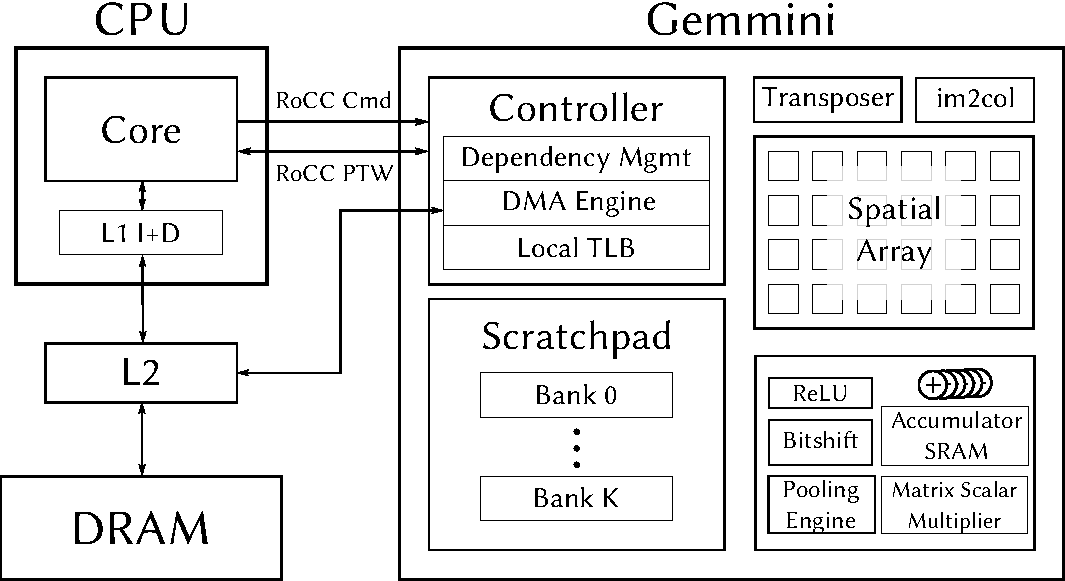
\includegraphics[width=0.9\linewidth]{fig/systolic_arch_system.pdf}
    \caption{Gemmini hardware architectural template overview.}
    \vspace{-0.3cm}
    \label{fig:arch-template}
    \vspace{-0.1in}
\end{figure}

%========OLD TEXT BELOW================

%\textcolor{red}{Introduce Gemmini here. Explain how it addresses the limitations earlier. In one concluding sentence, describe our performance/power.} Gemmini provides a push button flow from ONNYX representations to ready to tape-out design with all the necessary software and hardware libraries. It provides flexibility in the generated hardware and in the programming model allowing users to easily modify the underlying hardware configurations, add more hardware units and extend the ISA with new instructions. Gemmini also provides system level integration, and achieves comparable results to the industry standard NVDLA systolic array accelerator~\cite{}.

% Chipyard~\cite{chipyard} is a framework for designing and evaluating full-system hardware. It includes in-order, out-of-order RISC-V, and vector processors, and an accelerator for SHA3 hash function. In this work we extend the Chipyard framework with Gemmini: a systolic array generator.  A large portion of DNN accelerators produced by major vendors such as Google~\cite{tpu}, Samsung~\cite{samsung} and Tesla~\cite{bannon2019accelerated} have used systolic array architectures for matrix multiplication and convolution operations.

% Gemmini plugs-in within the tile interface of the Rocket Chip SoC generator ecosystem and the Chipyard integrated SoC research and development framework. As such, it integrates with a broad set of open-source heterogeneous SoC components and devices, including UARTs, GPIOs, JTAGs, shared-cache memory systems, and various accelerators. These components include the open-source SiFive inclusive L2 cache, the Hwacha vector accelerator [13], and BOOM.

%\textcolor{red}{Move this table and description of it to the Background section.} Figure~\ref{} shows the advantages of Gemmini as compared to NVDLA and VTA~\cite{} and where it is positioned in terms of flexibility, system level integration and performance.

% Gemmini is gaining widespread adoption in research labs. More than 30 students, both graduate and undergraduate, including ones with very little hardware experience, were able to take advantage of this in Berkeley's Hardware For Machine Learning class~\cite{} and design new features. In \cite{PekingTVM} Gemmini was integrated with TVM~\cite{TVM} allowing for automatic code generation and autotuning.

%\textcolor{red}{Describe case studies here, with one sentence each.} We perform three case studies on Gemmini and explore its flexibility, system-level integration, and performance (in terms of execution time, and energy consumption).
% Our evaluation includes booting Linux on Gemmini, running real cycle-accurate simulations on AWS FPGA instances using Firesim~\cite{karandikar2018firesim}, exploring multiple hardware configurations, programming models, and host co-processors and experimenting with a wide range of DNNs. 
%Finally, we fabricated two test systems-on-chip Gemmini designs in TSMC 16nm and Intel 22FFL process technologies.
%Our main contributions are:

% (programming model fine grained and coarse grained instructons and hardware), system level integration, comparable NVDLA + plot

% We have the whole package:
%     * push button flow from high level software to ready to tapeout flow.
%     * Software compilation
%     * Real system integration from
%     * FPGA-accelerated simulation to get cycle-accurate performance
%     * Physical design

%Hardware acceleration requires specialized hardware. The non-recurring
%engineering (NRE) costs of specialized hardware limit it's adoption to a small
%number of high-value applications. 
%%\textcolor{red}{Change this paragraph instead to focus on WHY we need generators.} With the demise of Dennard's scaling and the end of Moore's law, hardware customization became the go-to approach for handling the exacerbating compute demand. \textcolor{red}{Transition missing here, e.g. hardware customization is extremely difficult.} 
%Hardware generators~\cite{bora_generators, bora_generators2} are an attractive approach to lower the NRE costs of custom hardware. Rather than designing instances from scratch for each new application, designing highly-parameterized and modular instance generators which capture the main computational properties and control flow of hardware instances, but allow them to be tailored and customized to specific application use-cases. \textcolor{red}{(This previous sentence is too long. The discussion is also too general, so we should tie it closer to DNNs. Make a case for DNN generators in particular, rather than just generators.)}
%DNN accelerators are a prime use-case for hardware generators.
%Although DNN computational kernels may stay the same across workloads, characteristics such as layer dimensions or model size impact how workloads are optimally scheduled and mapped to any particular hardware accelerator, lending themselves to further accelerator customization. 
%By tailoring the parameters of a hardware generator to a target applications based on pre-silicon application-specific design-space-exploration, designer can extract maximal efficiency from an accelerator integrated with an application, while minimizing NRE costs for that particular application. 

%This paper describes the architecture and features of the Gemmini generator
%hardware and software tools together with a performance evaluation.

\section{Background and Motivation}\label{sec:motivation}

The demand for fast and efficient DNN execution from edge to cloud has led to a significant effort in developing novel accelerator instances that are
specialized for different DNN algorithms and/or different deployment scenarios.
% While such efforts have opened up new opportunities for DNN accelerators, they pose unique challenges in accelerator implementation, software ecosystem, and full-system integration of accelerators.
This section discusses recent advances in DNN accelerators and
DNN accelerator generators, motivating the need for a full-stack approach to
evaluate deep learning architectures.

\subsection{DNN Accelerators}

Researchers have proposed a large variety of novel DNN accelerators with different performance and energy efficiency targets for different applications across a diverse set of deployment scenarios~\cite{eyeriss2,shidiannao,scaledeep,moreau2018}. At the architecture level, different DNN accelerators exploit different reuse patterns to build specialized memory hierarchies~\cite{interstellar-asplos2020} and interconnect networks~\cite{maeri-asplos2018} to improve performance and energy efficiency. Most existing hardware DNN architectures are largely spatial, where parallel execution units are laid out spatially either in a systolic fashion, as in the case of the TPU, or in parallel vector units like Brainwave~\cite{brainwave-isca-2018} and NVDLA~\cite{nvdla-hotchips}. Based on these architectural templates, recent advances have also started exploring how to leverage applications' sparsity patterns~\cite{sigma-hpca2020,sparse-tpu,sparse-train} and/or emerging in-memory computing technology~\cite{pipelayer,algo-hardware-codesign-for-in-memory}.

\subsection{DNN Accelerator Generators}
Recent research has designed hardware generators % for general-purpose processors~\cite{Rocket-RISCV-2016} and, more recently,
for DNN accelerators~\cite{nvdla-hotchips,moreau2018,polysa,venkatesan2019magnet,dnnweaver,maeri-asplos2018}.
Table~\ref{tab:generator-comparison} compares the different features supported by existing hardware generators compared to Gemmini.
In contrast to building specific instances of hardware, generator-based
approaches provide parameterizable architectural
templates that can generate a wide variety of hardware and software instances, improving
hardware design productivity.
Here, we discuss the hardware, software, and system level requirements for DNN
accelerator generators to enable full-stack, systematic DNN architecture
evaluation.

DNN accelerator generators must provide flexible architectural templates to cover a wide variety of different DNN accelerator instances, each suited for a different execution environment and a different area/power/performance target. Most DNN accelerator generators today focus only on fixed-point representations and/or only support a single dataflow. In addition, today's generators only target a specific spatial array type, \textit{i.e.}, systolic-based (as in the TPU) or vector-based (as in NVDLA), making it challenging to systematically compare against them. In contrast, Gemmini supports 1) both floating and fixed point data types to handle data representations in training and inference, 2) multiple dataflows that can be configured at design time and run time, 3) both vector and systolic spatial array architectures, enabling quantitative comparison of their efficiency and scalability differences, and 4) direct execution of different DNN operators.
    
Moreover, DNN accelerator generators also need to provide an easy-to-use
programming interface so that end users can
quickly program their applications for the generated accelerators.
% This is of particular importance for the field of deep-learning research and
% development where new advances are happening almost every day, if not every
% hour.
Different developers would prefer different software design environments based upon their targets or research interests.
For example, DNN application practitioners would prefer that the hardware
programming environment be hidden by DNN development frameworks like
PyTorch or TVM so that they don't need to worry about low-level development
details, as in the case of VTA~\cite{moreau2018} and DNNWeaver~\cite{dnnweaver}.
At the same time, framework developers and system programmers may want to
interact with the hardware at a low level, in either C/C++ or assembly, to
accurately control hardware states and squeeze every bit of efficiency out, as in the case of MAGNet~\cite{venkatesan2019magnet} and Maeri~\cite{maeri-asplos2018}.
Unlike other DNN generators that tend to focus on one of these
requirements, Gemmini provides a multi-level programming interface
%with both C/C++ and ONNX~\cite{onnx}, an open exchange format built to represent DNN models across different frameworks,
to satisfy users with different requirements.
In addition, Gemmini is the first infrastructure that provides hardware support for virtual memory without the need for any special driver software, making it significantly easier for end-users to program accelerators.


%Finally, we would like to emphasize the importance of accelerator
Third, system-level integration, including both the SoC and the system software, is also critical in DNN accelerator generators.
Today's DNN accelerators are typically designed and evaluated in isolation. However, when they are eventually deployed, they need to be integrated as part of a larger system.
In fact, recent industry evaluations have demonstrated that modern ML
workloads could spend as much as 77\% of their time running on CPUs, even in the
presence of a hardware accelerator, to execute either new operators or to move
data between the CPU and accelerators~\cite{centaur-isca2020, edge-facebook,datacenter-facebook,ai-tax-hpca}.
% ~\cite{centaur-isca2020, edge-facebook,datacenter-facebook,ai-tax-hpca}.
However, unfortunately, none of the existing DNN accelerator generators support full SoC integration with host CPUs and shared resources like caches and system buses. Motivated by this observation, Gemmini has built-in system integration support where users can directly instantiate a complete SoC environment that can boot Linux, directly enabling architects to evaluate subtle trade-offs at the
system level.
%, which remain folded when viewing only the standalone accelerator block.

%There may be other subtle ways in which the full SoC or software stack impact
%performance, such as through cache contention or page evictions.
%A generator with full SoC and system integration makes it easier for architects
%to consider these trade-offs.

%=================OLD TEXT===============================
%One such generator is NVDLA~\cite{nvdla}, which can produce accelerators which
%target a variety of different ML kernels, sparsity techniques, and memory
%interfaces. By selecting different parameters, architects can produce
%accelerators that target low-power edge devices, or high performance servers,
%all using the same generator. Most of the hardware blocks that NVDLA is composed
%of can also optionally be taken out.

%However, the customizability of the individual hardware blocks is somewhat
%limited. For example, NVDLA's convolution engine is made up of a set of
%dot-product vector operators, but these can't be reconfigured by architects into
%a simple systolic array that would benefit from highly regular workloads.
%Additionally, NVDLA does not support full SoC integration on it's own; it
%instead produces hardware blocks that must be hooked up to the appropriate
%memory and system interfaces by the architect.

%MAGNet~\cite{venkatesan2019magnet} is another ASIC generator which provides a
%configurable HLS template as well as automated design-space-exploration tools
%which will tune this HLS template for specific neural networks such as ResNet50
%or AlexNet. However, the MAGNet project did not investigate full system
%integration, and nor does it describe a software stack, which is vital to
%running real workloads.

%PolySA~\cite{polysa} is another HLS-based generator. PolySA consumes C/C++ code
%describing algorithms to accelerate, and it then maps them to fixed systolic
%arrays. However, the work is focused primarily on the generation of the systolic
%arrays themselves, and so the full-system integration is not investigated.

%Prior work has also introduced VTA~\cite{moreau2018} and TVM~\cite{chen2018} as
%an integrated research platform for SW/HW evaluation of NN accelerators. VTA
%uses HLS to generate hardware accelerators while the TVM language is used to map
%operations onto them, providing an elegant programming interface. However, VTA
%does not target full SoC integration. The generator is also limited to integer
%datatypes, although many modern workloads, such as model training, require
%floating-point support



%For example, NeuFlow~\cite{neuflow} is a systolic-inspired architecture
%which supports a high degress of runtime configurability of individual
%processing elements (PEs). ShiDianNao~\cite{shidiannao} and
%Eyeriss~\cite{eyeriss}, similarly are composed of two-dimensional meshes, while
%also supporting broadcast and global connections between PEs and local
%scratchpads, which is not strictly systolic, but often improves performance.
%NVDLA~\cite{nvdla}, on the other hand, generates convolution engines composed of
%a one-dimensional set of parallel vector dot product trees. There are also many
%sparse accelerators based upon a variety of different architectures, such as
%Cambricon-X~\cite{} and SIGMA~\cite{}, whose parallel vector units contain
%different kinds of dot product reduction trees.

%%A large number of ML accelerator generators have been proposed, but existing
%solutions lack certain features that make them fully generalizable across all
%existing workloads and execution environments. For example, many existing
%solutions are specific instances of hardware, rather than parameterizable
%generators that can scale from the edge to the cloud. Many accelerators also
%lack full-system integration, from SoCs to system software, limiting their ease
%of use. We discuss some prior solutions in this section, as well as their
%limitations which are addressed by Gemmini. \textcolor{red}{(Preview the
%following two sections here and move this paragraph up into intro).}


% For example, NeuFlow~\cite{neuflow} is a systolic-inspired architecture which
% allows individual processing elements (PEs) to be re-configured at runtime to
% perform tasks such as multiply-accumulates, divisions, and non-linear
% activations. ShiDianNao~\cite{shidiannao}, similarly, allowed PEs, arranged in
% a two-dimensional mesh, to be reconfigured at runtime to perform
% multiply-accumulates, additions, and max poolings. 
% Eyeriss~\cite{eyeriss} implemented a weight-stationary dataflow using a
% spatial array. Eyeriss v2~\cite{eyeriss2} improved on the original Eyeriss by
% demonstrating a new PE architecture that can operate on sparse CSC-encoded
% matrices, and a hierarchical mesh NoC capable of unicast, multicast, and
% broadcast data transfers to maximize reuse.  These and other systolic-inspired
% architectures typically permit both global and local connections between PEs
% and global memory, which is not strictly systolic, but often improves
% performance.

% \textcolor{red}{Make this paragraph focus more on different environments.}
% Commercially deployed ASIC implementations of NN accelerators include the
% Google TPU \cite{tpu} for cloud workloads, as well as edge inference
% implementations by Samsung \cite{samsung}, Nvidia \cite{nvidia}, Apple
% \cite{apple}, and Tesla~\cite{bannon2019accelerated, bannon2019systems}
% \textcolor{red}{(replace these patents with the HotChips presentation)}, who's
% design is highly systolic. In particular, a detailed description of the
% original TPU implementation includes a $256\times256$ matrix multiplication
% unit implemented using a reduced-precision systolic MAC array with a weight
% stationary dataflow for NN inference in the cloud. Successor versions included
% floating-point representation, additional memory, and improved utilization for
% both training and inference~\cite{tpu2_3}.

% \textcolor{red}{(We would also need to cite Cambricon, Convoluton, SCNN, and
% other sparse accelerators). Mention that Cambricon-X and Convoluton were based
% on DianNao.} Accelerators targeting sparse workloads tend to be far less
% systolic, such as SIGMA~\cite{}, an accelerator which introduces a novel
% multiply-add reduction tree network within PEs, achieving high utilization on
% sparse GEMM workloads. In general, enabling sparse processing and mapping on
% accelerators that were not specifically targeted at sparse workloads requires
% much customization. \textcolor{red}{(Do we have a source for this? Can we
% mention that Eyeriss v2 targets sparse while Eyeriss v1 doesn't?)}

% \textcolor{red}{Reword: All of these architectures are tuned for different workloads/constraints. What we need is a generator that satisfies all of these requirements.} These accelerators were designed to accommodate significant runtime reconfigurations, especially the reconfiguration of connections between individual PEs, and between PEs and local memory. However, their architectures were quite fixed. \textcolor{red}{For example, they lacked the ability to switch between meshes of PEs performing scalar operations, and collections of PEs performing vector operations, even though both designs may be more suitable for different execution environments, physical design technologies, and workload types.} Thus, they provide highly efficient accelerators that work well for specific scenarios, but may not be suitable across all scenarios.

%\textcolor{red}{(We don't need one paragraph for each accelerator. Instead have 3 paragraphs for each requirement.)}

%\textcolor{red}{Make this three paragraphs} An ideal hardware generator would:

%\begin{enumerate}


%=================Table Playground======================
%\begin{table*}[]
%\centering
%\begin{tabular}{|l|ccccc|}
%\hline
% & \textbf{NVDLA} & \textbf{MAGNet} & \textbf{PolySA} & \textbf{VTA} & \textbf{Gemmini} \\ \hline
%\textit{Flexibility of architectural template} & $\times$ & $\times$ & $\times$ & $\times$ & \checkmark \\ \hline
%\textit{Programmability} & \checkmark & $\times$ & \checkmark & \checkmark & \checkmark \\ \hline
%\textit{Full SoC integration} & $\times$ & $\times$ & $\times$ & $\times$ & \checkmark \\ \hline
%\end{tabular}
%\caption{A comparison of various state-of-the-art hardware generators. \textcolor{red}{Are just $\times$'s and \checkmark's enough? Should ``Programmability'' be given a new name?}}
%\label{tab:motivation1}
%\end{table*}

%\begin{table*}[]
%\centering
%\begin{tabular}{|l|c|c|c|c|c|}
%\hline
% & \textbf{NVDLA} & \textbf{MAGNet} & \textbf{PolySA}  & \textbf{VTA} & \textbf{Gemmini} \\ \hline
%\textit{Flexibility} & \begin{tabular}[c]{@{}c@{}}Blocks can be removed,\\ but not customized\end{tabular} & \begin{tabular}[c]{@{}c@{}}Dataflows and dimensions\\ can be changed\end{tabular} & \begin{tabular}[c]{@{}c@{}}Arbitrary systolic\\ arrays supported\end{tabular} & \begin{tabular}[c]{@{}c@{}}GEMM instrinsics\\ can be modified\end{tabular} & \checkmark \\ \hline
%\textit{Programm.} & \begin{tabular}[c]{@{}c@{}}Comes with NVDLA\\ compiler\end{tabular} & $\times$ & \begin{tabular}[c]{@{}c@{}}HLS solution\\ for FPGAs\end{tabular} & \begin{tabular}[c]{@{}c@{}}Programmed\\ with TVM\end{tabular} & \checkmark \\ \hline
%\textit{Full SoC} & $\times$ & $\times$ & $\times$ & $\times$ & \checkmark       \\ \hline
%\end{tabular}
%\caption{A comparison of various state-of-the-art hardware generators. \textcolor{red}{(Attempt at a more full description)}}
%\label{tab:motivation2}
%\end{table*}

\vspace{-0.01in}
\section{Gemmini Generator}\label{sec:generator}
% \vspace{-0.05in}

% Gemmini is an open-source, full-stack generator of DNN accelerators, spanning across different architectures, programming interfaces, and system integration options. At the hardware level, Gemmini's architectural template is flexible enough to support a diverse set of numerical and structural microarchitecture parameters.
% In addition, Gemmini also produces software binaries tuned for each created hardware instance, either through a push-button programming interface via the ONNX Runtime~\cite{onnxruntime} or a low-level, Gemmini-provided Application Programming Interface (API) that is portable across Gemmini-generated accelerators.
% Programmers can target the provided API if they wish to write their own applications or create their own kernels.
% Finally, Gemmini generates not only accelerators, but full SoCs which can run real-world software stacks, including operating systems, during design space exploration. This enables architects to accurately evaluate the impact of the full SoC and software stack on efficiency and performance.

Gemmini is an open-source, full-stack generator of DNN accelerators, spanning across different hardware architectures, programming interfaces, and system integration options.
With Gemmini, users can generate everything from low-power edge accelerators to high-performance cloud accelerators equipped with out-of-order CPUs. Users can then investigate how the hardware, SoC, OS, and software overhead interact to affect overall performance and efficiency.

\subsection{Architectural Template}
\label{ssec:arch}

\begin{figure}[t]
    \centering
    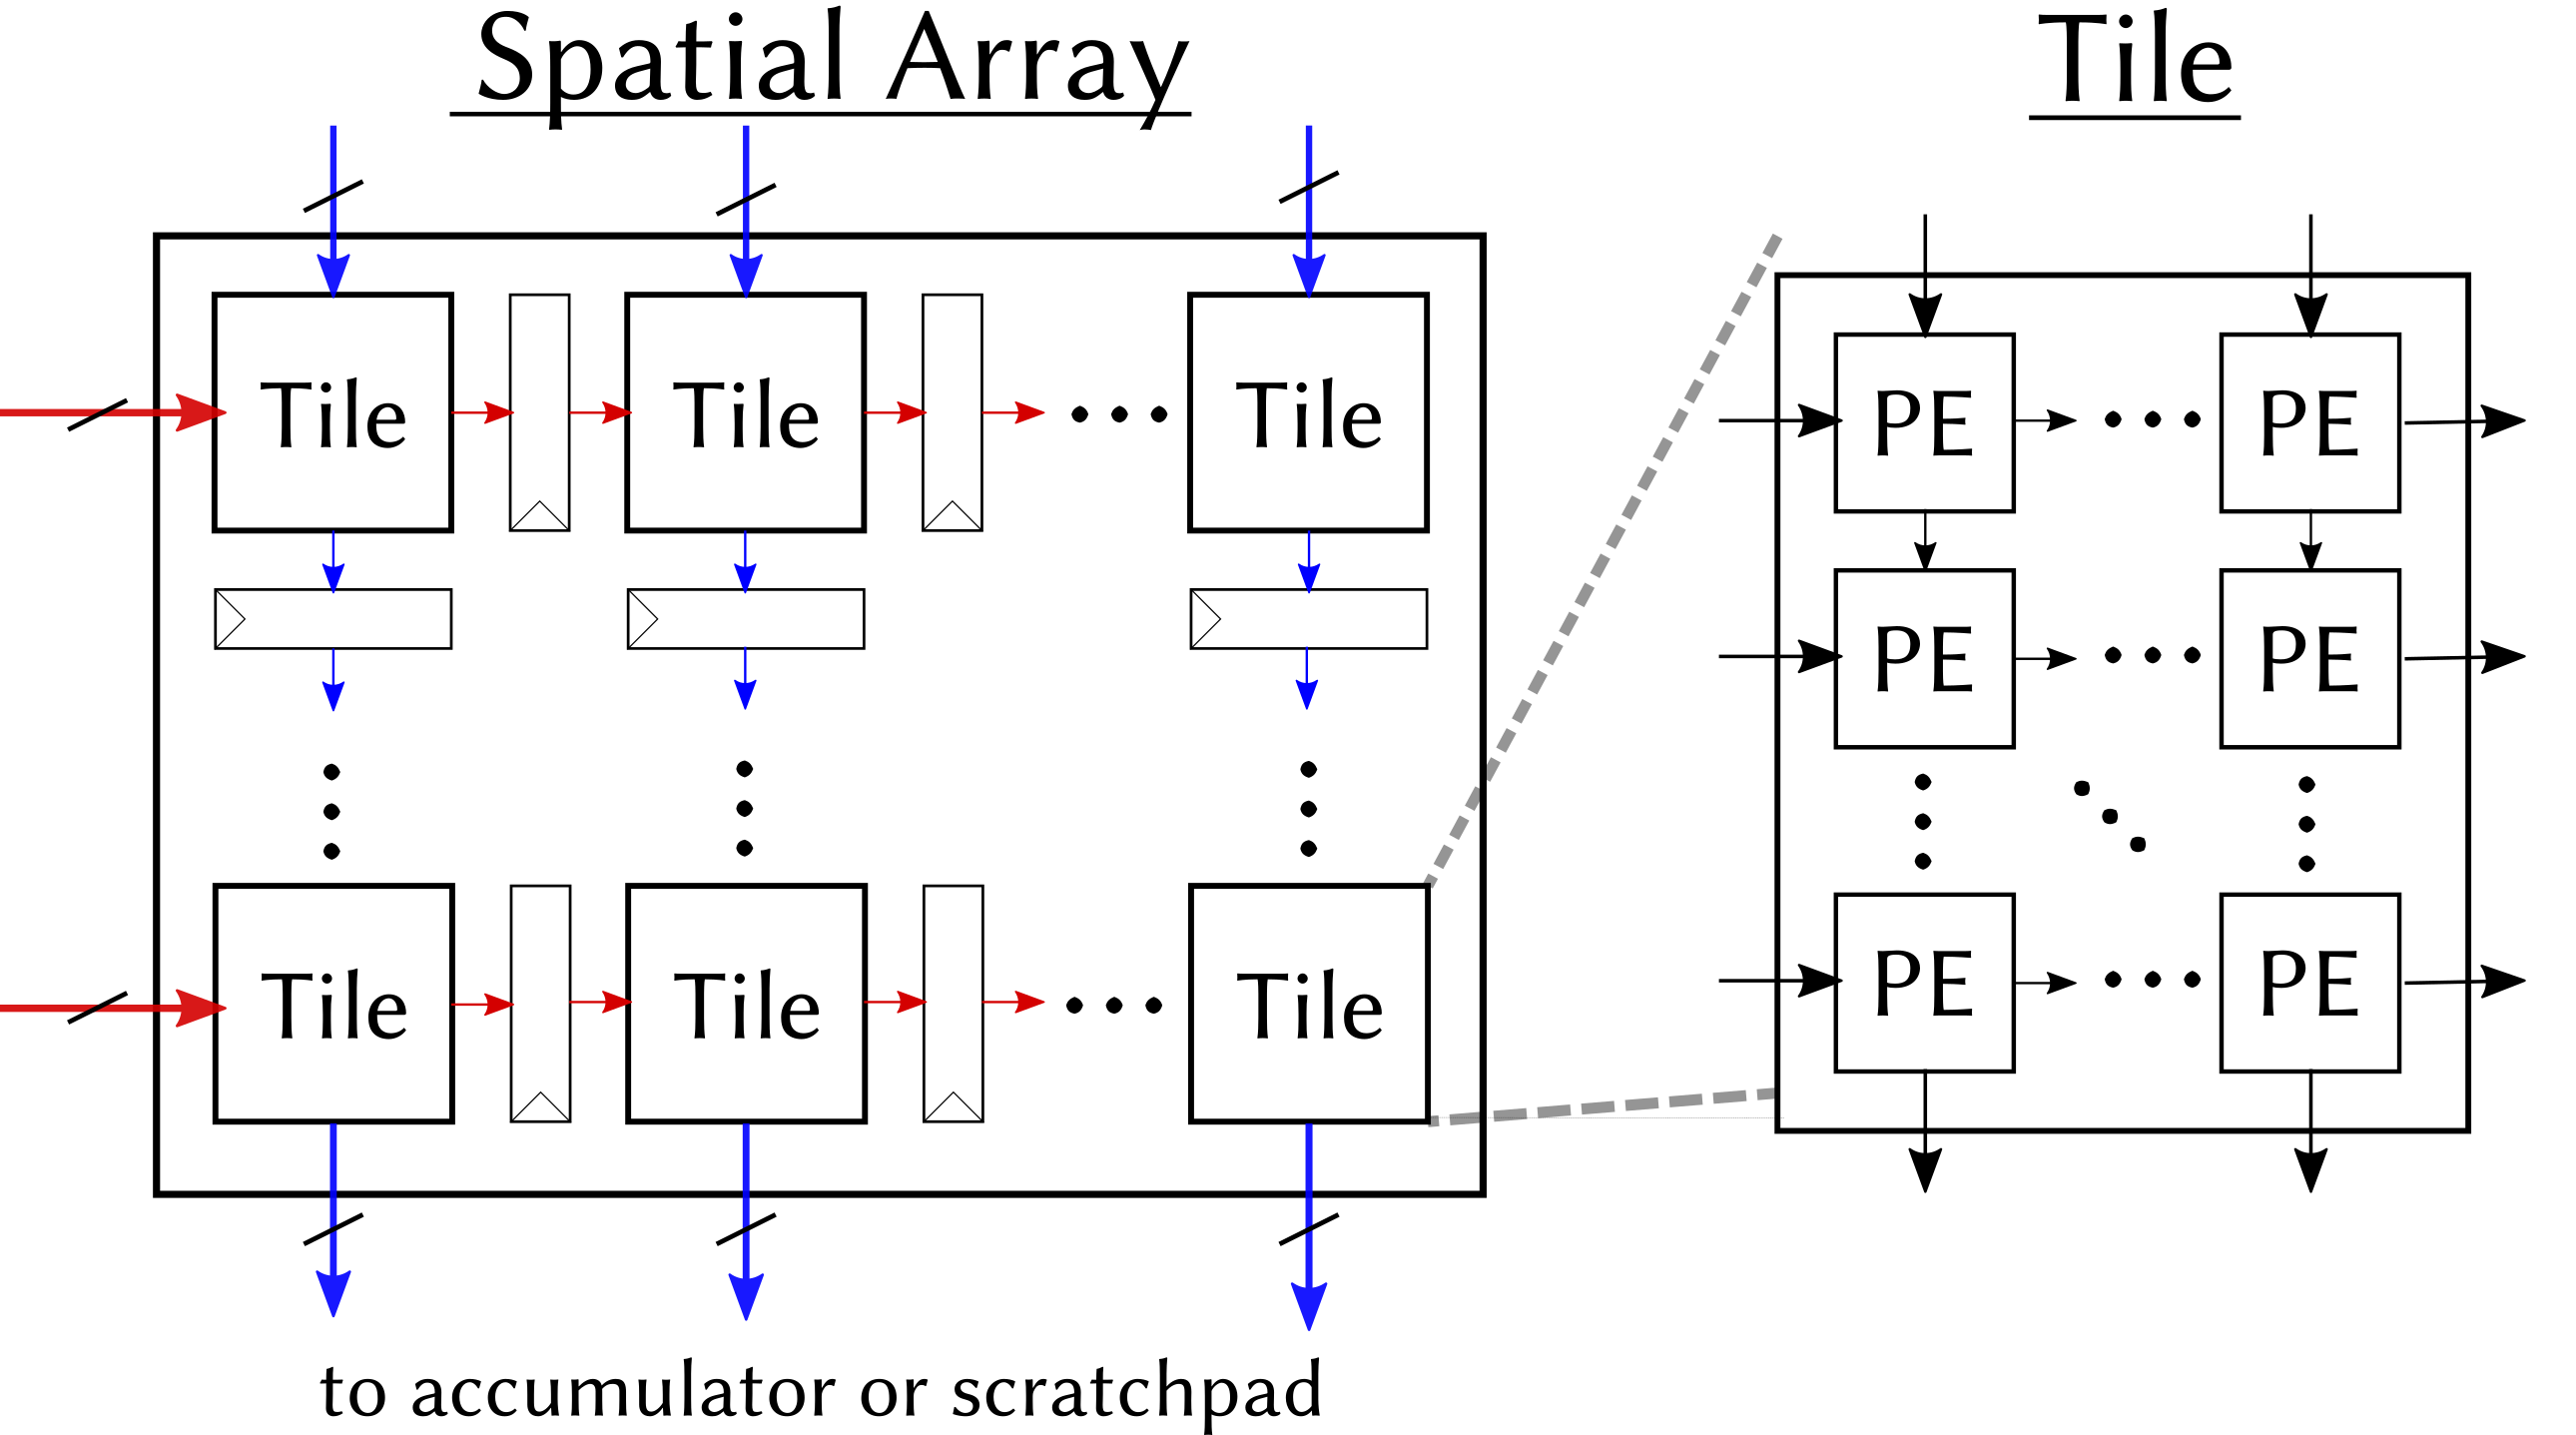
\includegraphics[width=0.85\linewidth]{fig/systolic_arch_detail3.png}
    \caption{Microarchitecture of Gemmini's two-level spatial array.} % The spatial array is composed of \textit{tiles}, connected via explicit, pipelined registers. Each tile can be further broken down into an array of \textit{Processing Elements (PEs)}, connected by a fully combinational grid.}
    \label{fig:systolic_arch}
    \vspace{-0.2in}
\end{figure}

Figure~\ref{fig:arch-template} illustrates Gemmini's architectural template.
The central unit in Gemmini's architectural template is a spatial architecture with spatially distributed processing elements (PEs), each of which performs dot products and accumulations.
The spatial array reads data from a local, explicitly managed scratchpad of banked SRAMs, while it writes results to a local accumulator storage with a higher bitwidth than the inputs.
Gemmini also supports other commonly-used DNN kernels, \textit{e.g.}, pooling, non-linear activations (ReLU or ReLU6), and matrix-scalar multiplications, through a set of configurable, peripheral circuitry.
Gemmini-generated accelerators can also be integrated with a RISC-V host CPU
to program and configure accelerators.

% \subsubsection{Spatial Array}

We design Gemmini's spatial array with a two-level hierarchy to provide a flexible template for different microarchitecture structures, as demonstrated in Figure~\ref{fig:systolic_arch}.
The spatial array is first composed of \textit{tiles}, where tiles are connected via explicit pipeline registers.
Each of the individual tiles can be further broken down into an array of PEs, where PEs in the same tile are connected combinationally without pipeline registers.
Each PE performs a single multiply-accumulate (MAC) operation every cycle, using either the weight- or the output-stationary dataflow.
The tiles are composed of rectangular arrays of PEs, where PEs in the same tile are connected combinationally with no pipeline registers in between them. The spatial array, likewise, is composed of a rectangular array of tiles, but each tile \textit{does} have pipeline registers between it and its neighbors.
Every PE and every tile shares inputs and outputs only with its adjacent neighbors.

Figure~\ref{fig:nvdla-vs-tpu-comparison} illustrates how Gemmini's two-level hierarchy provides the flexibility to support anything from fully-pipelined TPU-like architectures to NVDLA-like parallel vector engines where PEs are combinationally joined together to form MAC reduction trees, or any other design points in between these two extremes. We synthesized both designs with 256 PEs. We found that the TPU-like design achieves a 2.7x higher maximum frequency, due to its shorter MAC chains, but consumes 1.8x as much area as the NVDLA-like design, and 3.0x as much power, due to its pipeline registers. With Gemmini, designers can explore such footprint vs. scalability trade-offs across different accelerator designs.

\begin{figure}[t]
\centering
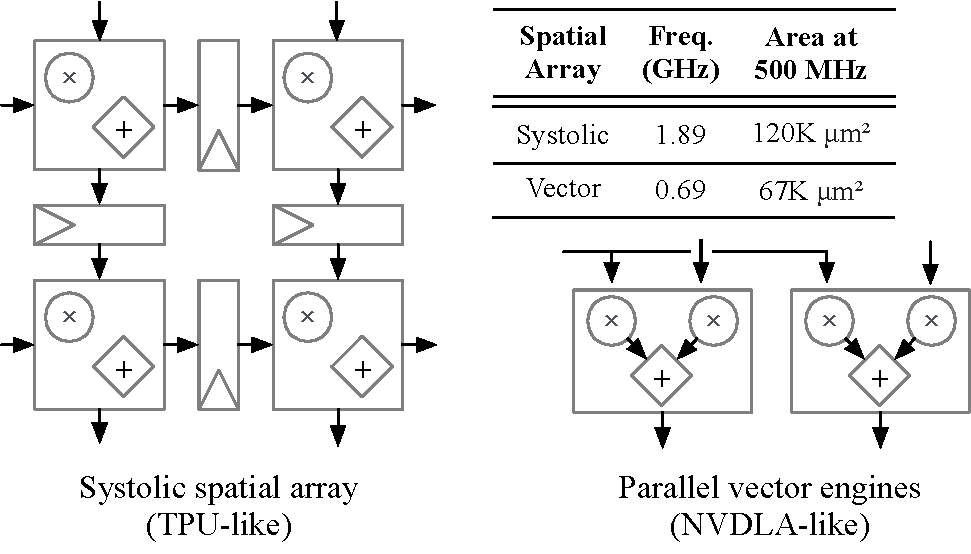
\includegraphics[width=\linewidth]{fig/Systolic-vs-NVDLA-smaller2.pdf}
\vspace{-0.2in}
\caption{Examples of two different spatial architectures generated by Gemmini. Both perform four multiply-accumulates per cycle though with different connectivities between multiply-and-accumulate units.}
\label{fig:nvdla-vs-tpu-comparison}
\vspace{-0.2in}
\end{figure}

% \begin{figure}[t]
% \centering
% \begin{subfigure}[b]{0.4\linewidth}
%     \centering
%     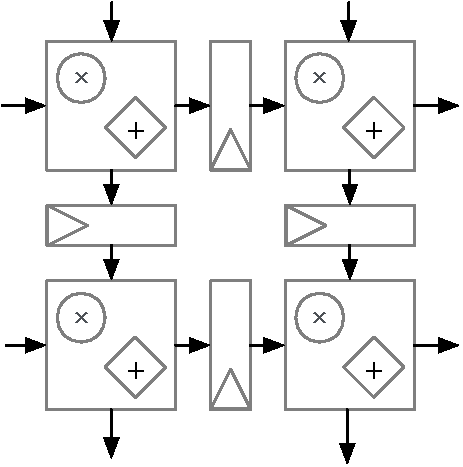
\includegraphics[width=\linewidth]{fig/tpu-like}
%     \caption{TPU-like spatial array with systolic processing.}
%     \label{fig:tpu-like}
% \end{subfigure}
% \hspace{0.05\linewidth}
% \begin{subfigure}[b]{0.45\linewidth}
%     \centering
%     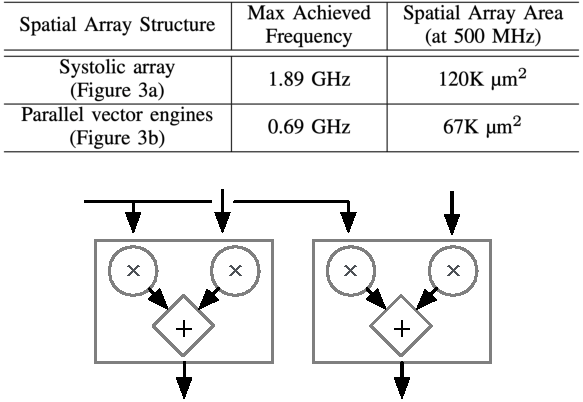
\includegraphics[width=\linewidth]{fig/NVDLA-smaller.pdf}
%     \caption{NVDLA-like spatial array with parallel vector engines.}
%     \label{fig:nvdla-like}
% \end{subfigure}
% \caption{Examples of two different spatial architectures generated by Gemmini. Both perform four multiply-accumulates per cycle though with different connectivities between multiply-and-accumulate units.}
% \vspace{-0.1in}
% \end{figure}

% These kinds of performance vs. footprint vs. scalability trade-offs must be decided by architects for any accelerator they design. Gemmini provides a unified framework with which they can generate and evaluate different architectures, making the design space exploration process simpler and easier.

% Table~\ref{tab:tpu-vs-nvdla} shows the maximum achieved frequency and area footprint of these two designs synthesized with Intel $22nm$ FinFET process.
% We notice that the systolic design achieves a 2.7$\times$ higher frequency than the parallel vector engines, as the extra pipeline registers greatly reduced the critical path lengths, demonstrating better scalability especially for larger array dimensions.
% %The is not unexpected, as systolic arrays are known to have strong scalability during physical design~\cite{}.
% At the same time, the extra pipeline registers also add significant area overhead of the systolic array, so that it consumes 1.8$\times$ more area compared to the parallel vector engines, and 3.0$\times$ as much power.

%These kinds of performance vs. footprint vs. scalability trade-offs must be decided by architects for any accelerator they design. Gemmini provides a unified framework with which they can generate and evaluate different architectures, making the design space exploration process simpler and easier.

% Gemmini supports this microarchitectural variation naturally by representing the spatial array as a two-level hierarchy. The inner dimension, which we call \textit{tiles}, is composed of combinationally-connected PE, where each PE performs a single multiply-accumulate operation per cycle. The outer dimension, which is the spatial array itself, is composed of tiles with pipeline registers between them. By tuning the sizes of the tiles within an array, architects can group individual PEs under the same combinational mesh, where they can be merged into dot-product reduction trees. Alternatively, limiting each tile to a size of only one PE produces a totally systolic design.

%\subsubsection{Parameters}

% \hl{Gemmini supports a large number of parameters, allowing a high degree of customization over the compute characteristics, memory capacity, and SoC-level characteristics of any accelerator that is generated. The most relevant parameters, described in Table~\mbox{\ref{tab:parameter-table}}, configure all parts of the compute stack, from the dataflow of the spatial array to the cache hierarchy of the host CPU and the main memory. For example, we can configure the datatype of the PEs to signed integers, unsigned integers, or floats, of any size defined by the user.}

% \begin{table}[t]
% \centering
% \begin{tabular}{l|c|c}
% \hline
% \makecell{Spatial Array Structure} & \makecell{Max Achieved\\Frequency} & \makecell{Spatial Array Area \\ (at 500 MHz)} \\ \hline\hline
% \makecell{Systolic array\\(Figure~\ref{fig:tpu-like})}          & 1.89 GHz               & 120K {\textmu}m$^2$       \\ \hline
% \makecell{Parallel vector engines\\(Figure~\ref{fig:nvdla-like})} & 0.69 GHz                & 67K {\textmu}m$^2$        \\ \hline
% \end{tabular}
% \caption{Maximum frequency and area footprint for two different Gemmini-generated spatial array architectures.}
% \vspace{-0.1in}
% \label{tab:tpu-vs-nvdla}
% \vspace{-0.1in}
% \end{table}

% \begin{table}[t]
% \begin{tabular}{ c | l | c }
% \hline
% \textbf{Category} & \textbf{Parameter} &  \textbf{Recommended Range} \\  
% \hline
% \hline
% \multirow{5}{*}{\makecell{Spatial\\Array}} & Mesh Rows & 1--256 \\
% & Mesh Columns & 1--256 \\
% & Tile Rows  & 1--256  \\
% & Tile Columns  & 1--256  \\
% & Dataflow & \makecell{Weight/Output stationary,\\or both} \\
% \hline
% \multirow{4}{*}{\makecell{\makecell{Accelerator\\Memory}}} & Scratchpad Capacity & 256 bytes--16 MB \\
% & Accumulator Capacity  & 256 bytes--8 MB  \\
% & Scratchpad Banks  & 1--4 \\
% & Accumulator Banks  & 1--4 \\
% \hline
% \multirow{3}{*}{\makecell{\makecell{Execution\\Schedule}}} & ROB Entries & 4--128 \\
% & Load Queue Entries & 2--128 \\
% & Store Queue Entries & 2--128\\
% & Execute Queue Entries & 4--128 \\
% \hline
% \multirow{4}{*}{\makecell{\makecell{Controller}}} & PE Latency & 0--4 cycles \\
% & DMA Bus Width & 64--256 bits \\
% & DMA Block Size & 32--64 bytes \\
% & TLB Entries & 2--64 \\
% \hline
% \multirow{4}{*}{\makecell{\makecell{Datatypes}}} & Datatype & SInt/UInt/Float/User-defined \\
% & Input Bitwidth & 8--32 bits \\
% & Output Bitwidth & 8--32 bits \\
% & Accumulator Bitwidth & 16--64 bits \\
% \hline
% \multirow{3}{*}{\makecell{\makecell{Operators}}} & Multiply by Scalar & Present/Not \\
% & Transposer & Present/Not \\
% & Pooling & Present/Not \\
% & Im2col & Present/Not \\
% \hline
% \multirow{6}{*}{\makecell{\makecell{System}}} & Host Processor\footnote{Each host processor has a long list of potential parameters associated with it} & Rocket, BOOM \\
% & Number of Cores & 1-64 \\
% & Number of Accelerators & 0-Number of Cores \\
% & Shared L2 Cache Size & 256 KB -- 16 MB \\
% & Peripherals & UART, GPIO, SPI, JTAG, etc. \\
% & IO Models & \makecell{Network, DDR3, Block Device\\Latency-Bandwidth pipeline} \\ 
% \hline
% \end{tabular}
% \caption{Gemmini hardware configurable parameters. For the integer ranges, all power-of-2 values between the maximum and minimum are permitted. All parameters are independent of each other, and the size of the total search space is the cross-product of all possible parameter values. \textcolor{red}{HASAN: Cut table 3 in half.}}
% \label{tab:parameter-table}
% \end{table}

% \hl{\textbf{Optional compute blocks:} Peripheral compute blocks also exist to support non-linear activation functions, max-pooling, transpositions, and im2col. These blocks can be optionally left out of the generator to save area and power consumption for workloads that do not require them. The im2col block allows us to support both convolutions and matrix multiplications efficiently with the same spatial array.} \textcolor{red}{Should we mention the optional compute blocks?}

% \hl{The presence or absence of these blocks can significantly affect the performance and memory requirements of Gemmini applications at runtime. For example, if the im2col module is \textit{not} instantiated, then the Gemmini-generated accelerator will not be able to perform arbitrary convolutions directly on the input data. Instead, it will first map those convolutions to matrix multiplications through the im2col~\mbox{\cite{chetlur2014cudnn}} operation, which runs on the CPU and duplicates data, causing a significant memory expansion. Those im2col-ed buffers are then fed into the Gemmini-generated accelerator's local scratchpad increasing memory storage requirements and saturating the memory bandwidth.}

% \hl{
% However, if the im2col block \textit{is} instantiated, then Gemmini will instead run a seven-nested convolution loop directly, without requiring the host CPU to shuffle and duplicate data. Instead, the im2col module within the accelerator will repeatedly fetch the same pieces of data and feed them multiple times into the spatial array. Therefore, the duplication essentially happens \textit{in time} in the interface between the local scratchpad and the spatial array, rather than happening \textit{in space} in local or main memory.
% We demonstrate the performance impact of using the im2col module over running im2col on the host CPU in Section~\mbox{\ref{sec:evaluation}}.
% }

% \subsubsection{Im2Col}

% \hl{
% We demonstrate the operation of the im2col block in Figure~\mbox{\ref{fig:im2col}}. The im2col module is essentially an address generator which repeatedly fetches the same scratchpad entries across different matrix multiplications. The programmer only specifies the dimensions of the convolution operator (e.g. kernel width, image height, etc.) and the im2col block then generates all the (potentially non-contiguous) scratchpad addresses necessary to perform a convolution on the accelerator.
% }

% \begin{figure}[h]
%     \vspace{-0.2cm}
%     \centering
%     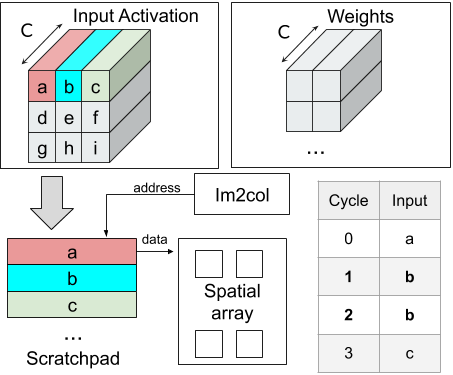
\includegraphics[width=0.7\linewidth]{fig/im2col.png}
%     \caption{Operation of im2col block, showing when different entries in the scratchpad are fed into the spatial array. Notice how the same row of the input activations, $b$, is fed into the spatial array multiple times. In cycle 1, $b$ is fed into the PEs on the first row of the spatial array, and in cycle 2, $b$ is fed into the PEs on the second row of the spatial array.}
%     \label{fig:im2col}
%     \vspace{-0.15in}
% \end{figure}

\subsection{Programming Support}
\label{software}

The Gemmini generator produces not just a hardware stack, but also a tuned software stack, boosting developers' productivity as they explore different hardware instantiations.
Specifically, Gemmini provides a multi-level software flow to support different programming scenarios.
At the \textit{high level}, Gemmini contains a push-button software flow which reads DNN descriptions in the ONNX file format
% ~\cite{onnx}
and generates software binaries that will run them, mapping as many kernels as possible onto the Gemmini-generated accelerator. Alternatively, at the \textit{low level}, the generated accelerator can also be programmed through C/C++ APIs, with tuned functions for common DNN kernels. These functions must be tuned differently for different hardware instantiations in order to achieve high performance, based on scratchpad sizes and other parameters. Therefore, every time a new accelerator is produced, Gemmini also generates an accompanying header file containing various parameters, \textit{e.g.} the dimensions of the spatial array, the dataflows supported, and the compute blocks that are included (such as pooling, im2col, or transposition blocks).

\begin{figure}[t]
    \centering
    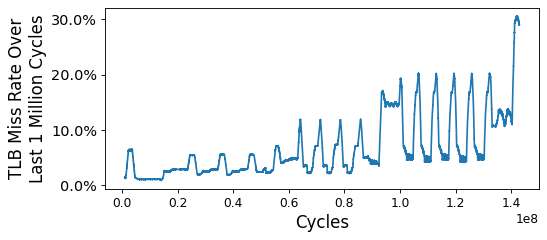
\includegraphics[width=\linewidth]{fig/tlb_hit_rate_running.png}
    \caption{TLB miss rate over a full ResNet50 inference, profiled on a Gemmini-generated accelerator.}
    \label{fig:tlb_hit_rate}
    \vspace{-0.2in}
\end{figure}

\textbf{Data Staging and Mapping:}
At runtime, based on the dimensions of a layer's inputs, and the hardware parameters of the accelerator instantiation, Gemmini uses heuristics to maximize the amount of data moved into the scratchpad per iteration.
Gemmini calculates loop tile sizes at runtime, and these tile sizes determine when and how much data is moved between DRAM, L2, and scratchpad during the execution of our tiled matrix multiplication, convolution, residual-addition, etc. kernels.
If the programmer wishes, the low-level API also allows them to manually set tile-sizes for each kernel.
% This runtime tuning is transparent to the programmer so that they can call the same DNN kernel functions to offload tasks onto different Gemmini-generated accelerators even if they were parameterized differently, without any porting or re-programming effort required.

\textbf{Virtual Memory Support:}
In addition to the programming interface, Gemmini also makes it easier to program accelerators by providing virtual memory support. This is useful for programmers who wish to avoid manual address translations as well as for researchers who wish to investigate virtual memory support in modern accelerators.
Gemmini also enables users to co-design and profile their own virtual address translation system. For example, Figure~\ref{fig:tlb_hit_rate} shows the miss rate of an example accelerator's local TLB profiled on Gemmini. As we can see, the miss rate occasionally climbs to 20-30\% of recent requests, due to the tiled nature of DNN workloads, which is orders-of-magnitude greater than the TLB miss rates recorded in prior CPU non-DNN benchmarks~\cite{lustig2013tlb}.
Later, in Section~\ref{virtual-memory-case-study}, we use Gemmini to co-design a virtual address translation system which achieves near-maximum end-to-end performance on accelerated DNN workloads, with only a few TLB entries in total.

\subsection{System Support}
\label{system}

% Gemmini supports full SoC integration, as well as evaluation on a realistic software stack including OS overheads, through its integration with the Chipyard SoC framework~\cite{chipyard}.
% Using Chipyard, Gemmini parameterizes not only the accelerator itself, but also the host CPU, memory interconnects, main memory cache hierarchy, and other system-level parameters.
% These components can be elaborated, interconnected, evaluated with a real software stack including operating-system overheads, and pushed through VLSI implementation flows~\cite{Hammer}, all within the unified Chipyard environment. 
% Cycle-exact simulations can run on the FPGA-accelerated FireSim~\cite{karandikar2018firesim} platform, even when evaluating large, complex SoCs running entire operating systems alongside compute-intensive workloads.

%\subsubsection{SoC Parameters}

%Gemmini provides a number of SoC parameters which modify the SoC outside the accelerator itself.
%We describe here some of these parameters and their potential impact on performance and efficiency.

%\textbf{Host CPU (Single- and Multi-Core):} 
Gemmini allows architects to integrate RISC-V CPUs % which supports the RoCC interface~\cite{Rocket-RISCV-2016}
with Gemmini-generated accelerators in the Chipyard~\cite{chipyard} framework.
These can range from simple, in-order microcontrollers which are not expected to do much more than IO management, all the way up to out-of-order, high-performance, server-class CPUs that may be running multiple compute-intensive applications even as they are sending commands to the Gemmini-generated accelerator.
% As DNN models evolve, some host CPUs may be required to complete execute operations and control flow that are not supported by Gemmini, increasing their impact upon overall performance.
SoCs can also be configured to host \textit{multiple} host CPUs and Gemmini-generated accelerators, which can each operate on different tasks in parallel with each other. Figure~\ref{fig:contention-soc} is one example of a dual-core system, where each CPU has its own Gemmini-generated accelerator.
Additional SoC-level parameters include bus widths between accelerators and host CPUs, as well as the size, associativity and hierarchy of the caches in the multicore, multicache memory system. Later, in Section~\ref{cache-contention}, we show how these parameters can be tuned, based on the computational characteristics of DNNs, to improve performance by over~8\%.

\begin{figure}[t]
     \centering
     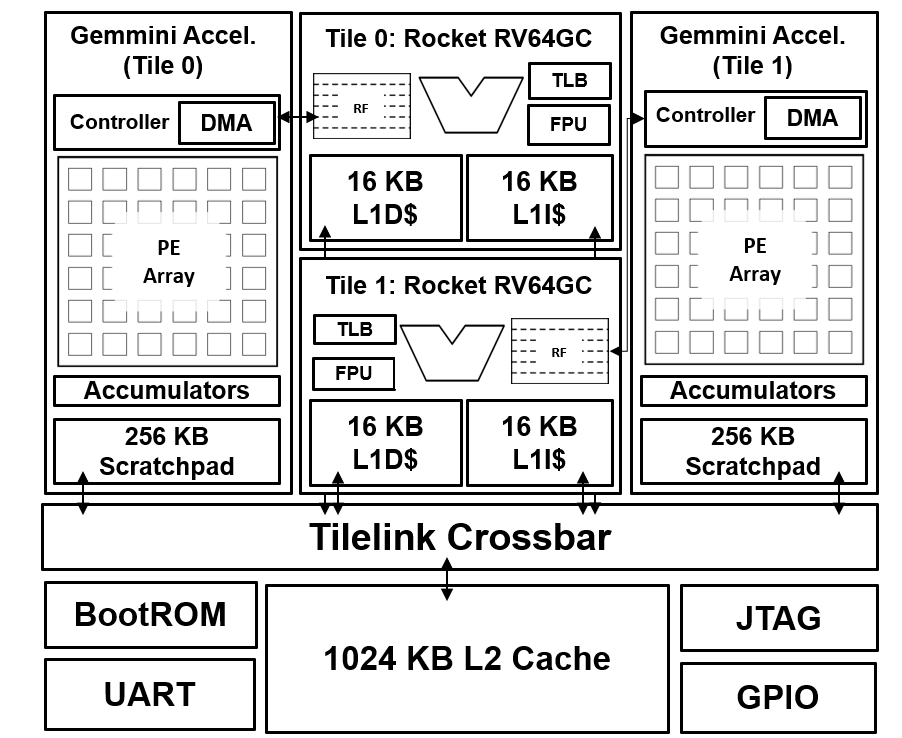
\includegraphics[width=0.75\linewidth]{fig/contention-soc.png}
     \caption{Example dual-core SoC with a Gemmini accelerator attached to each CPU, as well as a shared L2 cache and standard peripherals.}
     \label{fig:contention-soc}
     \vspace{-0.2in}
 \end{figure}

RISC-V-based full SoC integration also enables deep software-stack support, such that Gemmini-generated accelerators can easily be evaluated running the full software stack up to and including the operating system itself. This enables early exploration of accelerated workloads in a realistic environment where context switches, page table evictions, and other unexpected events can happen at any time. These unexpected events can uncover bugs and inefficiencies that a ``baremetal'' environment would not bring to the surface. For example, our experience of running Linux while offloading DNN kernels to a Gemmini-generated accelerator uncovered a non-deterministic deadlock that would only occur if context switches happened at very particular, inopportune times.
Running on a full software stack with an OS also uncovered certain bugs where Gemmini read from certain regions of physical memory without the proper permissions. On a ``baremetal'' environment, these violations were silently ignored.


\section{Gemmini Evaluation}\label{sec:evaluation}
This section discusses our evaluation methodology and evaluation results of Gemmini-generated accelerators compared to both CPUs and state-of-the-art, commercial accelerators.

\subsection{Evaluation Methodology}

We evaluate the end-to-end performance of Gemmini-generated accelerators using the FireSim FPGA-accelerated simulation platform~\cite{karandikar2018firesim}. We evaluate five popular DNNs: ResNet50, AlexNet, SqueezeNet v1.1, MobileNetV2, and BERT.
All DNNs are evaluated with a full Linux environment on a complete cycle-exact simulated SoC.
We synthesize designs using Cadence Genus with the Intel 22nm FFL process technology and place-and-route them using Cadence Innovus.
Our layout and area breakdown, described in Figure~\ref{fig:evaluation}, show that the SRAMs alone consume 67.1\% of the accelerator's total area. The spatial array itself only consumes 11.3\%, while the host CPU consumed a higher 16.6\% of area.

% We evaluated the end-to-end execution performance of Gemmini-generated accelerators on five commonly-used DNN workloads: ResNet50, AlexNet, SqueezeNet v1.1, MobileNetV2, and BERT.
% All the DNNs were evaluated with a full Linux environment on a complete cycle-exact simulated SoC, using the FireSim FPGA-accelerated simulation platform~\cite{karandikar2018firesim}.
% Additionally, for our physical design, we synthesized accelerators using Cadence Genus with the Intel 22nm FFL process technology and placed-and-routed them using Cadence Innovus.
% Our layout is illustrated in Figure~\ref{fig:area-layout}, and our area breakdown, described in Figure~\ref{tab:area-table}, shows that the SRAM memories alone consumed 67.1\% of the accelerator's total area. The spatial array itself only consumed 11.3\%, while the host CPU consumed a higher 16.6\% of area.

\subsection{Performance Results}

We evaluated the performance of several Gemmini configurations, with different host CPUs and different ``optional'' compute blocks, to determine how the accelerator and host CPU configuration may interact to impact end-to-end performance. In particular, we evaluated two host CPUs: a low-power in-order Rocket core, and a high-performance out-of-order BOOM core. We used two different Gemmini configurations:
one \textit{without} an optional im2col block, and the other \textit{with} an im2col block which allowed the accelerator to perform im2col on-the-fly, relieving the host CPU of that burden.

As illustrated in Figure~\ref{fig:perf-dnn}, when the accelerator is built without an on-the-fly im2col unit, its performance depends heavily on the host-CPU which becomes responsible for performing im2col during CNN inference.
A larger out-of-order BOOM host CPU increases performance by 2.0x across all CNNs.
The less complex the DNN accelerator is, the more the computational burden is shifted onto the CPU, giving the host CPU a larger impact on end-to-end performance.

\begin{figure}[t]
% \centering
\begin{subfigure}[b]{0.5\linewidth}
\centering
\scalebox{0.8} {
\begin{tabular}{ l | r | r }
\hline
\textbf{Component size} &  \textbf{\makecell{Area\\($\mu m ^2$)}} & \textbf{\makecell{\% of \\System\\Area}} \\
\hline
\hline
Spatial Array (16x16) & 116K & 11.3\% \\
Scratchpad (256 KB) & 544K & 52.9\%  \\
Accumulator (64 KB) & 146K & 14.2\%  \\
% Gemmini Control & 51K & 3.1\% \\
% \hline
% Total (Gemmini) & 858K & 52.5\% \\
% \hline
CPU (Rocket, 1 core) & 171K & 16.6\% \\
% Shared L2 (512 KB) &  534K & 32.7\%  \\
% Buses and Peripherals & 70K & 4.3\%  \\
\hline
% Total (Overall) & 1,632K & 100.0\% \\
Total & 1,029K & 100.0\% \\
\hline
\end{tabular}
}
\caption{Area breakdown.}
\label{tab:area-table}
\end{subfigure}
\hfill
\begin{subfigure}[b]{0.4\linewidth}
\centering
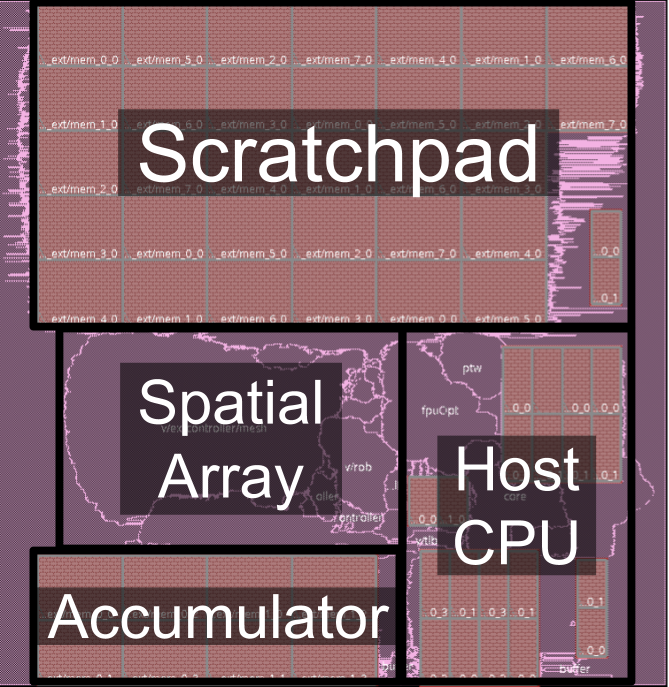
\includegraphics[width=0.8\linewidth]{fig/pnr.png}
\caption{Layout.}
\label{fig:area-layout}
\end{subfigure}
% \begin{subfigure}[b]{0.45\linewidth}
% \centering
% 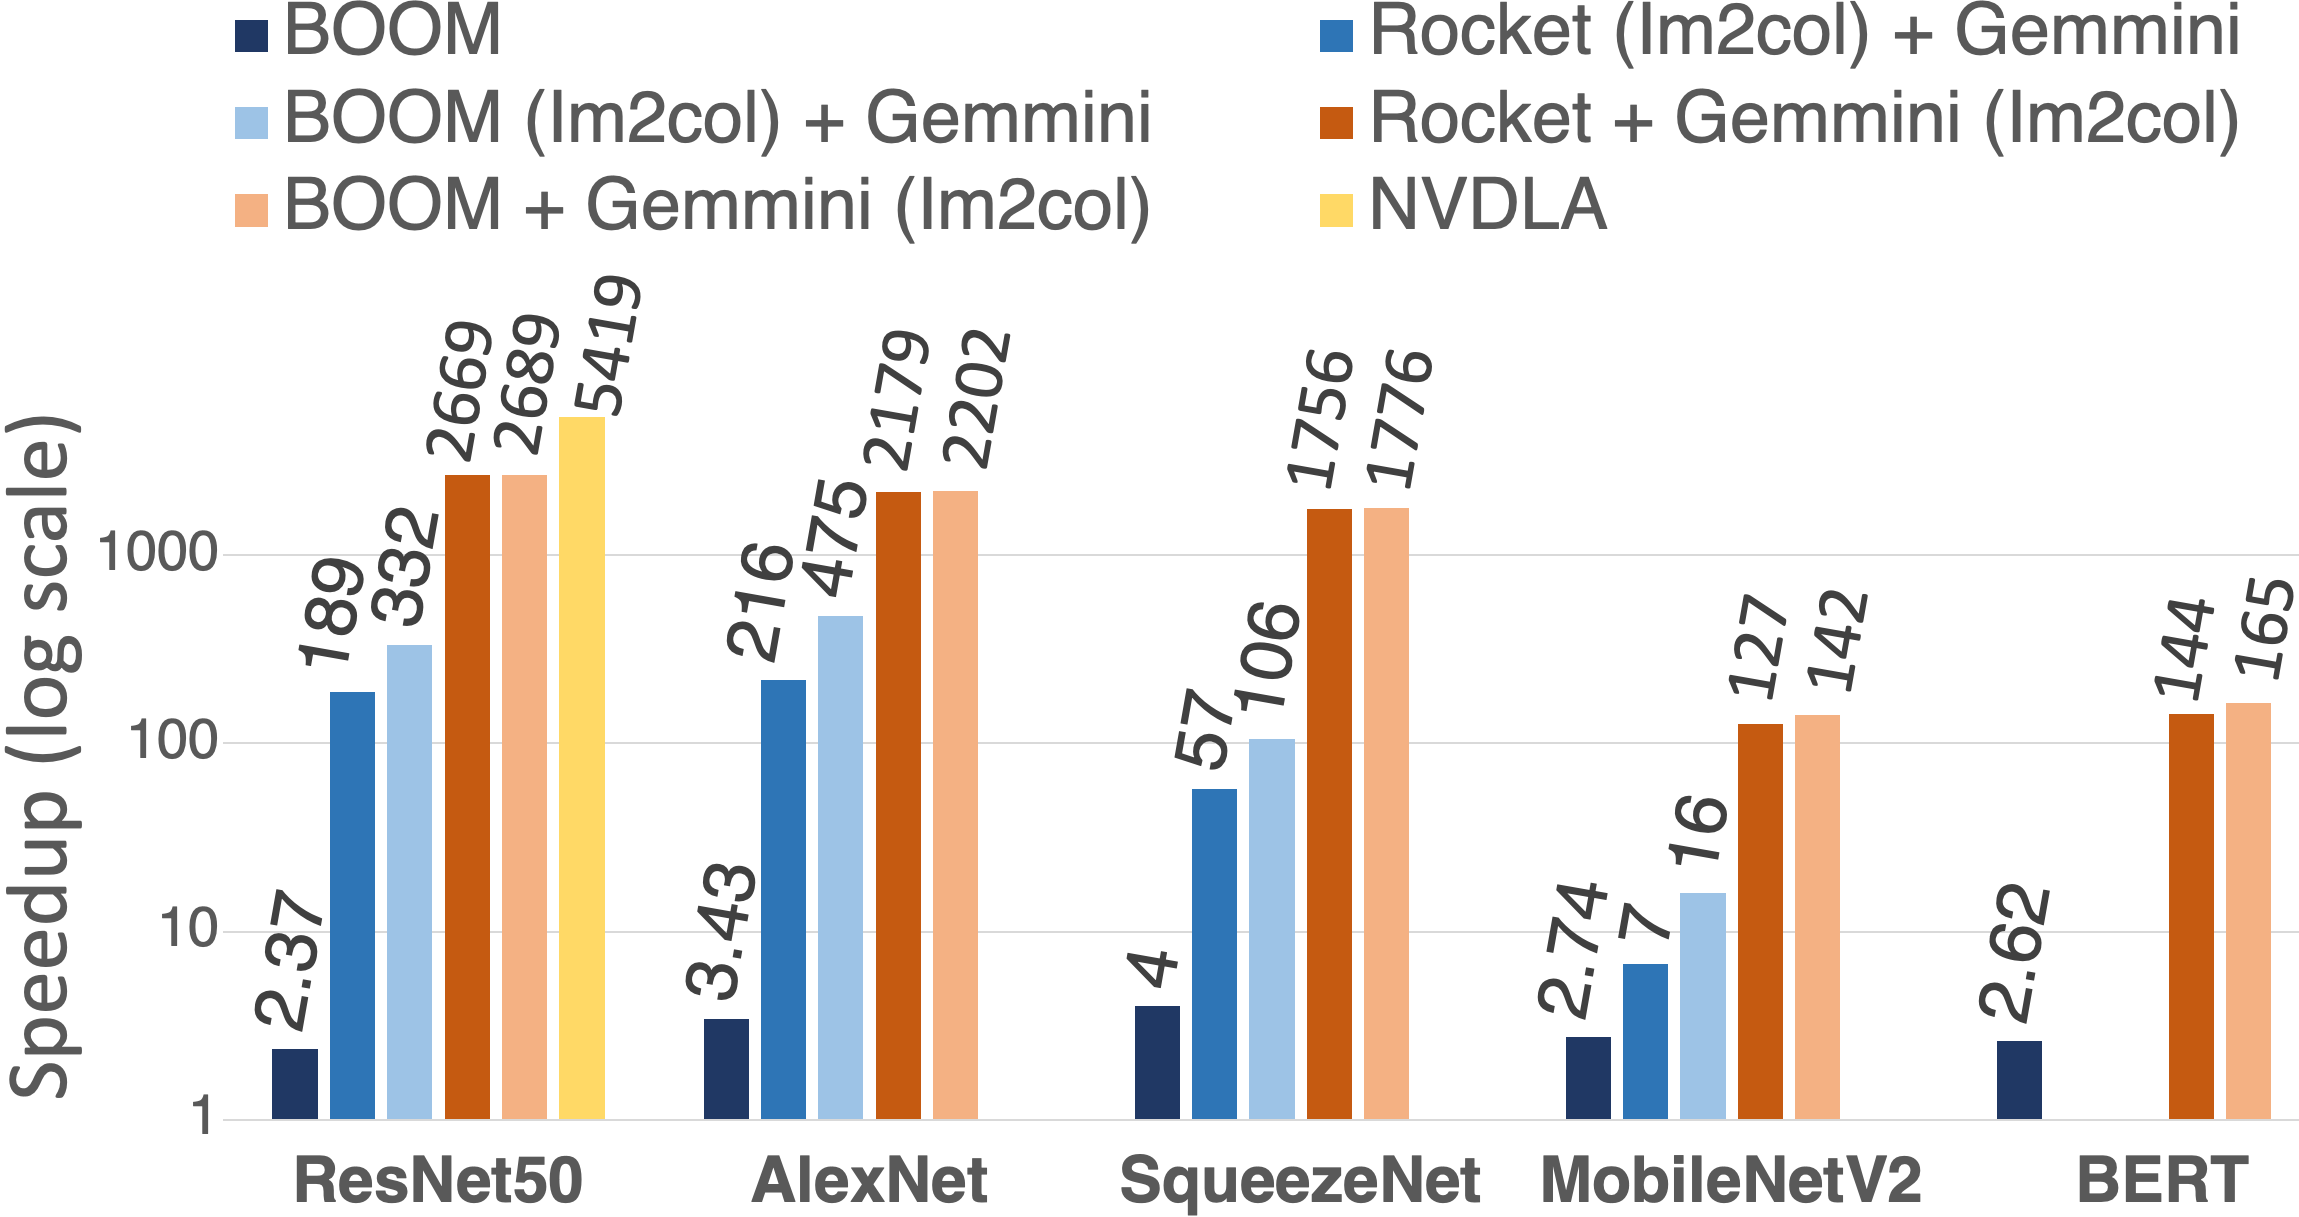
\includegraphics[width=\linewidth]{fig/perf-conv-new.png}
% \caption{Performance compared to an in-order CPU baseline. For CNNs, im2col was performed on either the CPU, or on the accelerator.}
% \label{fig:perf-dnn}
% \end{subfigure}
\caption{Area breakdown and layout of accelerator with host CPU.}
\label{fig:evaluation}
\vspace{-0.2in}
\end{figure}

\begin{figure}[b]
\centering
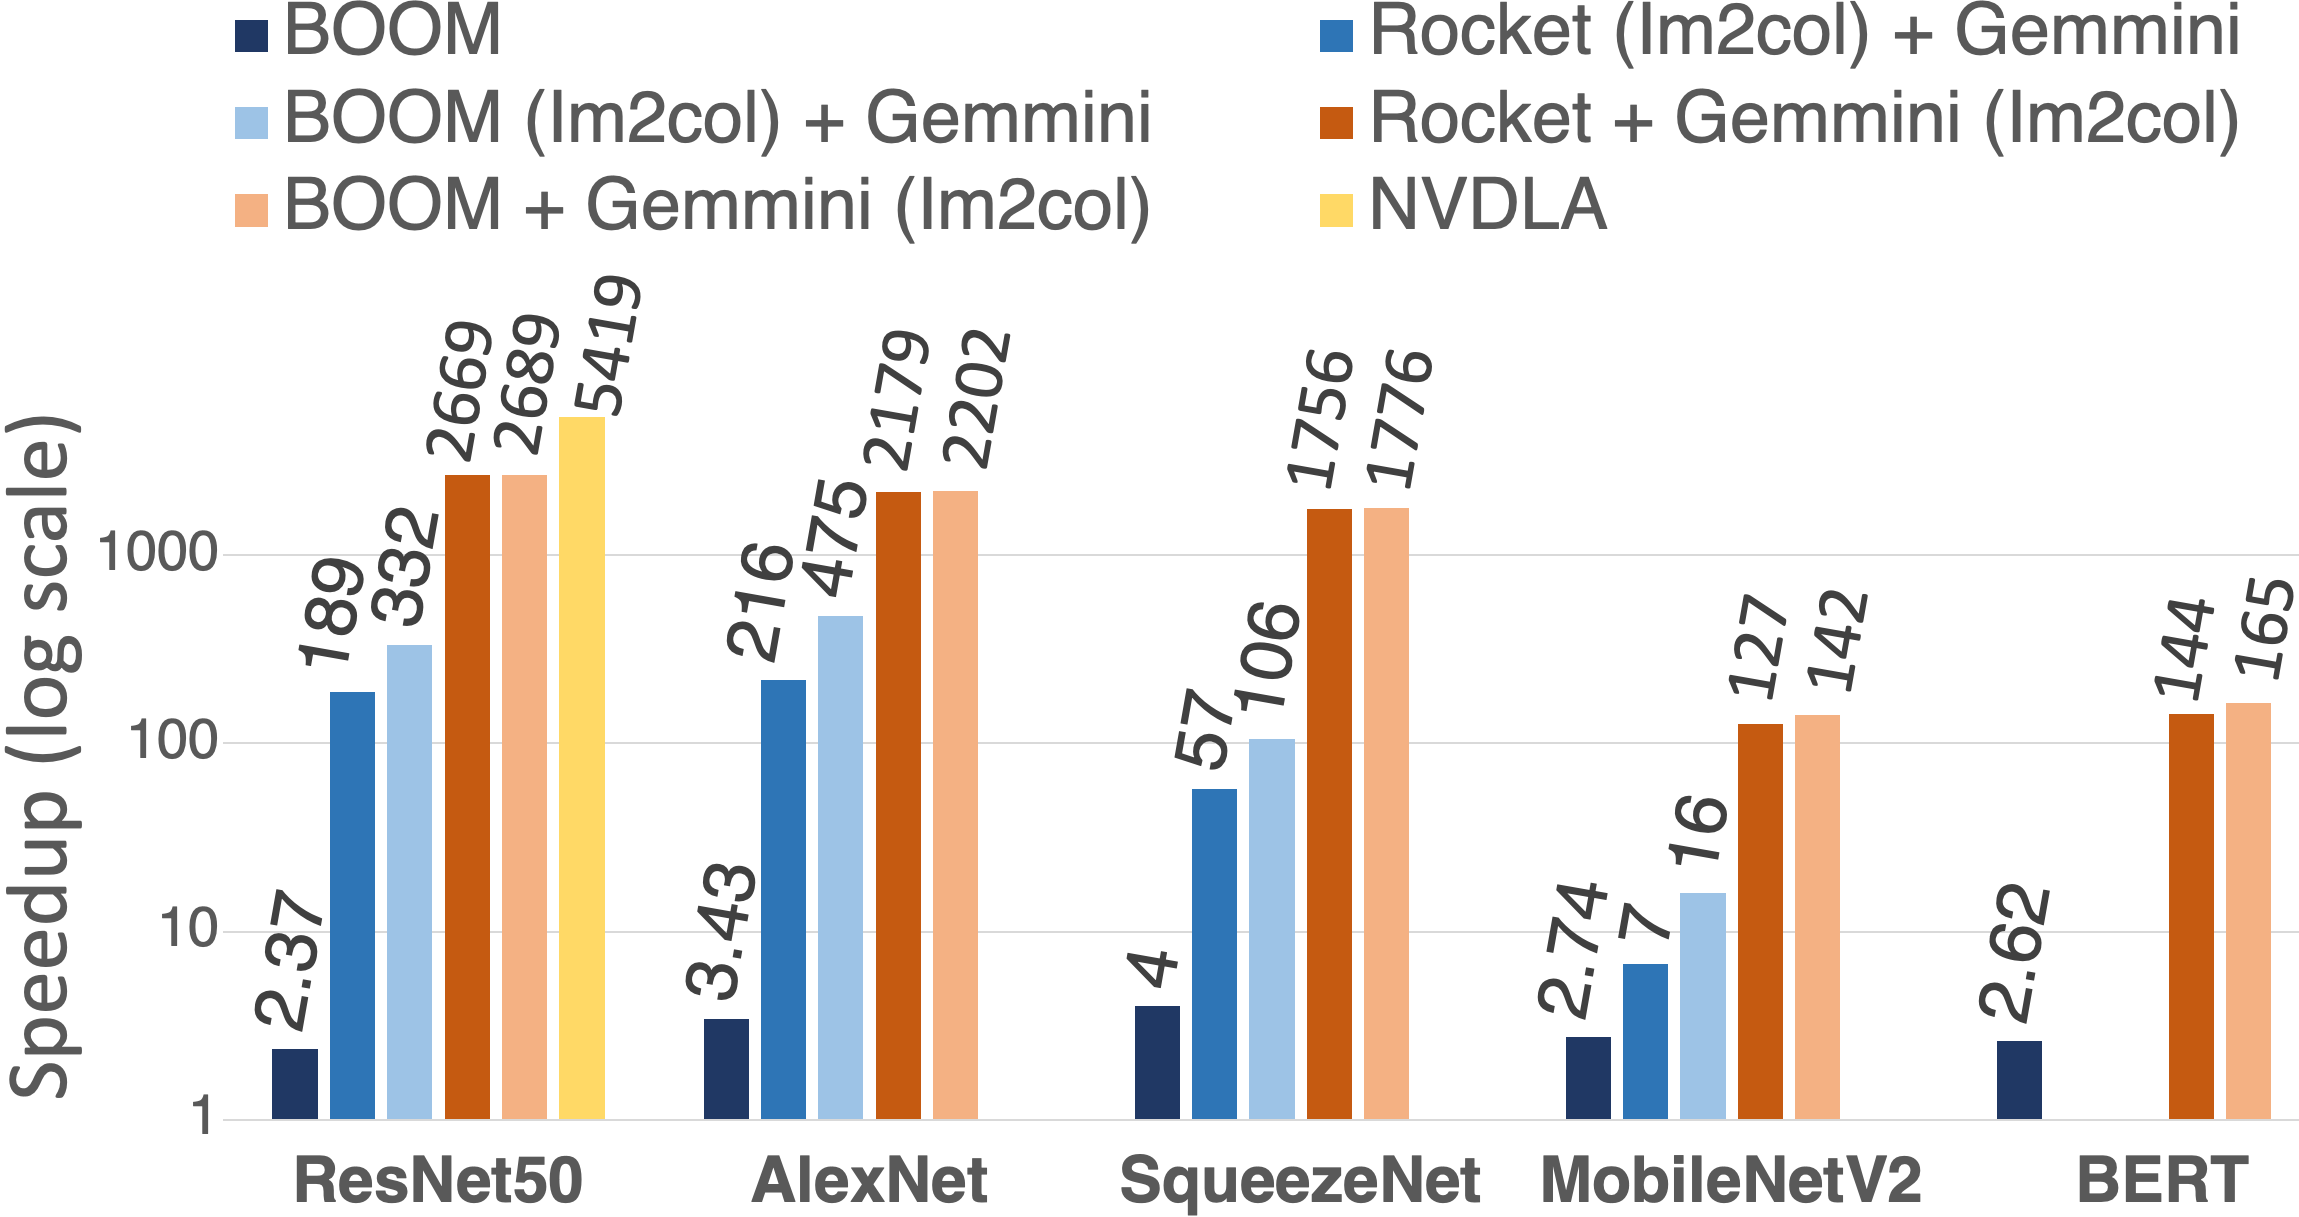
\includegraphics[width=\linewidth]{fig/perf-conv-new.png}
\caption{Speedup compared to an in-order CPU baseline. For CNNs, im2col was performed on either the CPU, or on the accelerator.}
\label{fig:perf-dnn}
\end{figure}

However, when the accelerator is equipped with an on-the-fly im2col unit, the choice of host CPU is far less important, because the CPU's computational burden is shifted further onto the accelerator. Adding a small amount of complexity to the accelerator allows us to reduce the area and complexity of the host CPU to a simple in-order core while preserving performance. Gemmini enables hardware designers to easily make these performance-efficiency tradeoffs.

With the on-the-fly im2col unit and a simple in-order Rocket CPU, Gemmini achieves 22.8 frames per second (FPS) for ResNet50 inference when running at 1 GHz, which is a 2,670x speedup over the in-order Rocket CPU and an 1,130x speedup over the out-of-order BOOM CPU. The accelerator also achieves 79.3 FPS on AlexNet. Some DNN models such as MobileNet are not efficiently mapped to spatial accelerators due to the low data reuse within the depthwise convolution layers. Therefore, Gemmini demonstrates only a 127x speedup compared to the Rocket host CPU on MobileNetV2, reaching 18.7 FPS at 1GHz.  On SqueezeNet, which was designed to be run efficiently on modern CPUs while conserving memory bandwidth, Gemmini still demonstrates a 1,760x speedup over the Rocket host CPU. Our results are comparable to other accelerators, such as NVDLA, when running with the same number of PEs as the configuration in Figure~\ref{tab:area-table}. When running language models such as BERT, Gemmini achieves a 144x improvement over the Rocket CPU.

% \textbf{Comparison to other accelerators:} Additionally, Figure~\mbox{\ref{fig:perf-dnn}} plots the performance of the state-of-the-art NVDLA accelerator~\mbox{\cite{nvdla-perf}},
% for those DNNs which NVDLA has published results for, as a comparison point with our Gemmini-generated accelerator. However, NVDLA's performance numbers came from an analytical model released by NVIDIA, rather than by actually running on an NVLDA instance comparable to our Gemmini-generated accelerator.
% Our results are comparable to other commercial accelerators which were tested with real hardware, such as the Kirin 970 NPU, which achieves 21.9 FPS on ResNet50, as compared to 23 FPS on our Gemmini-generated accelerator, with similar hardware resources~\mbox{\cite{kirin-perf}}.

% \begin{figure}[t]
% \centering
% 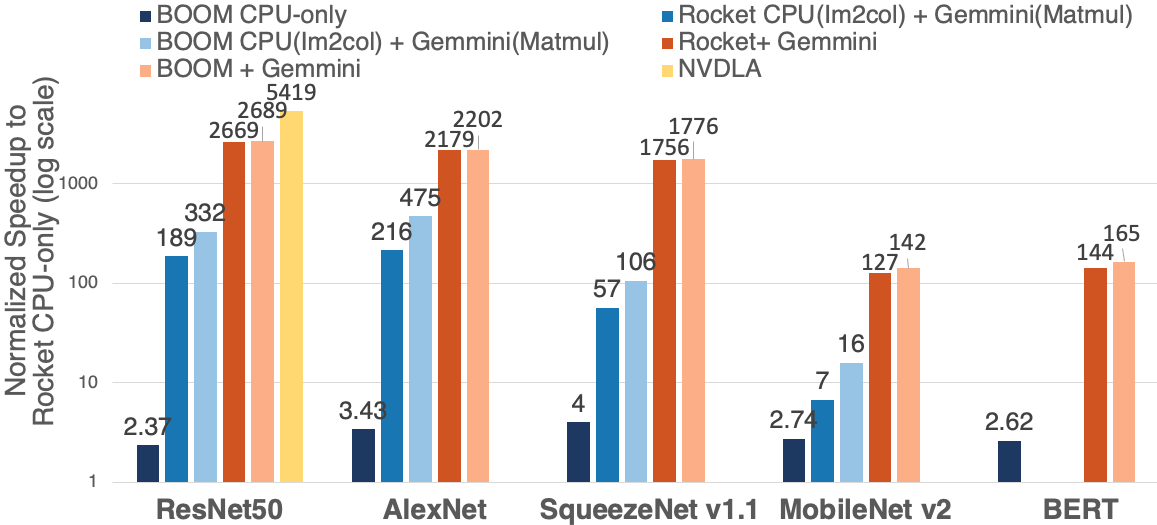
\includegraphics[width=0.95\columnwidth]{fig/perf-conv.png}
% \caption{Performance evaluation of Gemmini-generated accelerators with and without the im2col hardware module compared to a CPU baseline and NVDLA published performance. BERT has no convolutions, so im2col is not run as part of it.}
% \label{fig:perf-dnn}
% \vspace{-0.4cm}
% \end{figure}

% \textcolor{red}{Gemmini's does not reach NVDLA's performance is because the im2col block achieves low utilization on layers with few input channels, such as the RGB first layer input to our CNNs. Overlap between memory and compute instructions is also not as high as it could be due to a mismatch between the granularity of the memory and compute ISA instructions. This mismatch causes the Gemmini-generated accelerator's ROB to fill with instructions that cannot begin execution. Both these performance maladies are currently being rectified, and we expect our performance to improve closer towards NVDLA's baseline when they do.}


% According to \cite{nvdla-perf}, NVDLA reported both ResNet and AlexNet results by selecting the maximum value between DRAM communication cycles and MAC computation cycles for each layer and summing them. Furthermore, both numbers are made by numerical scaling from 2048 MAC / 512KB case.  This would mean they have assumed perfect overlap between data movement from/to DRAM and MAC computation, and perfect scaling, which might be optimistic. On the other hand, our results are from real end-to-end cycles, which captures any non-overlapped cycles between data movement and mesh operation as well as CPU code execution cycles, such as calculating tiling factors and iterating over nested loops by generated tiling factors.

%\footnote{AlexNet inference results for NVDLA are published only for the 2048 MAC / 512 KB configuration. Therefore, we divide that result by 8 in order to estimate against the equivalent Gemmini/NVDLA configuration}






%\section{Case Study: System-Level \\ Integration}
\section{Gemmini Case Studies}\label{sec:casestudies}
This section demonstrates how Gemmini enables full system co-design with two case studies. We use Gemmini to design a novel virtual address translation scheme, and to find the optimal SoC-level resource partition scheme of a multi-core, multi-accelerator system.

\subsection{Virtual Address Translation}
\label{virtual-memory-case-study}

% Point of this paragraph: We need a framework to co-design accelerators together with the virtual memory system.
With an RTL-level implementation that supports virtual memory, users can co-design their own virtual address translation schemes based on their accelerator and SoC configuration. Prior works in virtual address translation for DNN accelerators have proposed very different translation schemes, from NeuMMU~\cite{neummu-asplos2020}, which calls for a highly parallel address-translation system with 128 page-table walkers (PTWs), to Cong et al.~\cite{address-trans-cong-hpca2017}, who recommend a more modest two-level TLB hierarchy, with the host CPU's default PTW co-opted to serve requests by the accelerator. This lack of convergence in the prior literature motivates a platform that allows co-design and design-space exploration of the accelerator SoC together with its virtual address translation system, for both hardware designers and researchers. Fortunately, with Gemmini, we can iterate over a variety of address translation schemes as we tune the accelerator and SoC.

% Point of this paragraph: Describe our experimental setup
To demonstrate, we configure Gemmini to produce a two-level TLB cache, with one private TLB for the accelerator, and one larger shared TLB at the L2 cache that the private TLB falls back on when it misses. Our design includes only one PTW, shared by both the CPU and the accelerator, which is suitable for low-power devices. We configure the accelerator for low-power edge devices, with a 16-by-16 systolic mesh and a 256 KB scratchpad. As shown in Figure~\ref{fig:tlb_wait_cycles}, we iterate over a variety of TLB sizes to find the design that best balances TLB overhead and overall performance, including over a design point where the shared L2 TLB has zero entries.

% Point of this paragraph: The private TLB gives you much more bang-for-your-buck than the L2 TLB.
Figure~\ref{fig:tlb_wait_cycles} demonstrates that the private accelerator TLB has a far greater impact on end-to-end performance than the much larger shared L2 TLB. Increasing the private TLB size from just four to 16 improves performance by up to 11\%. However, adding even 512 entries to the L2 TLB never improves performance by more than 8\%. This is because our workloads exhibit high page locality; even with tiled workloads, our private TLB's hit rate remained above 84\%, even with the smallest TLB sizes we evaluated. In fact, we found that 87\% of consecutive \textit{read} TLB requests, and 83\% of consecutive \textit{write} TLB requests, were made to the same page number, demonstrating high page locality. However, because reads and writes were overlapped, read and write operations could evict each other's recent TLB entries.

\begin{figure}
    \centering
    \begin{subfigure}[t]{0.439\linewidth}
        \centering
        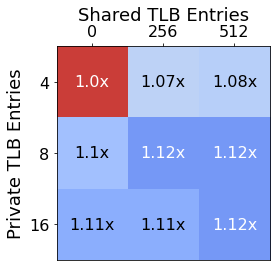
\includegraphics[width=\linewidth]{fig/tlb_entries.png}
        \caption{Without filter registers.}
        \label{fig:tlb_wait_cycles}
    \end{subfigure}
    \hfill
    \begin{subfigure}[t]{0.439\linewidth}
        \centering
        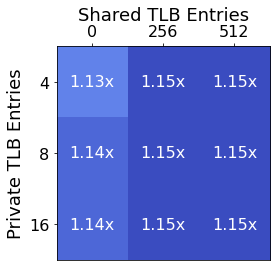
\includegraphics[width=\linewidth]{fig/tlb_entries_with_filter.png}
        \caption{With filter registers.}
        \label{fig:tlb_wait_cycles_with_filter}
    \end{subfigure}
    \caption{Normalized performance of ResNet50 inference on Gemmini-generated accelerator with different private and shared TLB sizes.}
    \vspace{-0.2in}
\end{figure}

% Point of this paragraph: On top of tuning the TLB sizes, we can make small optimizations to the virtual address translation system.
Although tuning TLB sizes improves hit rates, our private TLB hit latency in the tests shown in Figure~\ref{fig:tlb_wait_cycles} was still several cycles long. Fortunately, using the Gemmini platform, we were able to implement a simple optimization: a single register that caches the last TLB hit for read operations, and another register that caches TLB hits for write operations. These two registers allow the DMA to ``skip'' the TLB request if two consecutive requests are made to the same virtual page number, and help reduce the possibility of read-write contention over the TLB. These ``filter registers'' reduce the TLB hit latency to 0 cycles for consecutive accesses to the same page. As Figure~\ref{fig:tlb_wait_cycles_with_filter} shows, this low-cost optimization significantly improves our end-to-end performance, especially for small private TLB sizes. Due to our high TLB hit rate and low TLB hit penalty, we found that a very small 4-entry private TLB equipped with filter registers, but without an expensive shared L2 TLB, achieved only 2\% less than the maximum performance recorded. With such a configuration, the private TLB hit rate (including hits on the filter registers) reached 90\% and further increases to either TLB's size improved performance by less than 2\%, even if hundreds of new TLB entries were added.
% the total number of cycles spent by the DMA waiting for a TLB response only reached \textcolor{red}{X\%} of the total end-to-end runtime, showing that the virtual address translation scheme was no longer a primary performance bottleneck.

Using Gemmini, we have demonstrated that a modest virtual address translation system, with very small private TLBs, a single page-table-walker, and two low-cost filter registers for the TLB, can achieve near maximum performance for low-power edge devices. Gemmini is designed to enable such co-design of the SoC and its various components, such as its virtual address translation system.


\subsection{System-Level Resource Partition}
\label{cache-contention}

%We have better system-level integration than anyone else. There is a push-button flow to generate RTL for an entire SoC, including a RISC-V CPU, a TileLink interconnect, cache hierarchy, etc.

%This system-level integration allows us to perform an apples-to-apples comparison to state-of-the-art accelerators like NVDLA, to whom we will \textbf{hopefully} be competitive by publication time.

%Gemmini uses the RoCC interface of the Rocket Chip
%SoC generator and a TileLink memory port to communicate with a host processor system. Gemmini is also a part of Chipyard integrated SoC research
%and development framework~\cite{chipyard}, which provides it with a broader digital design environment which includes additional IP components, FPGA-accelerated simulation using the FireSim~\cite{karandikar2018firesim} platform, and VLSI implementation flows. The integration with the Chipyard enables a broad spectrum of high fidelity evaluation and experimentation with Gemmini.

% \textbf{Paragraphs:}
% \begin{enumerate}
%     \item Gemmini enables application-system co-design.
%     \item Real-world DNN applications, such as ResNet50, have diverse layer types which react to system configurations in different ways
%     \item Experimental setup
%     \item As shown in Figure X, layers with higher arithmetic intensity benefit more from a bigger scratchpad. Memory-bound layers, like resadds, are unaffected in the single-core case
%     \item However, in the dual core case, residual addition layers benefit very much from higher cache sizes
%     \item This demonstrates that memory partitioning schemes must be co-designed with the application in order to achieve maximum performance.
% \end{enumerate}

% Point of this paragraph: Gemmini enables application-system co-design.

Gemmini also enables application-system co-design for real-world DNN workloads. To demonstrate, we present a case study describing a system-level design decision: memory partitioning based on application characteristics. We investigate memory partitioning strategies in both single-core and multi-core SoCs.

% Point of this paragraph: Real-world DNN applications, such as ResNet50, have diverse layer types which react to system configurations in different ways

\begin{figure*}[t]
\centering
\begin{subfigure}[b]{0.325\textwidth}
    % \vspace{23pt}
    \centering
    \scalebox{0.875} {
    \begin{tabular}{ l | c | c | c }
    \hline
    \makecell{Config\\Name} & \makecell{Scratchpad\\(per core)} & \makecell{Accumulator\\(per core)} & \makecell{L2\\Cache} \\  
    \hline
    \hline
    Base & 256 KB & 256 KB & 1 MB   \\
    BigSP & 512 KB & 512 KB & 1 MB  \\
    BigL2 & 256 KB & 256 KB & 2 MB  \\ \hline
    \multicolumn{1}{c}{} & \multicolumn{1}{c}{} & \multicolumn{1}{c}{} & \multicolumn{1}{c}{} \\
    \end{tabular}
    }
    \caption{Resource contention SoC configurations}
    \label{tab:contention-soc-configs}
\end{subfigure}
\hfill
\begin{subfigure}[b]{.325\textwidth}
    \vspace{0pt}
      \centering
      % include first image
      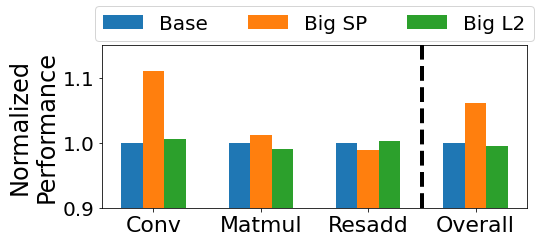
\includegraphics[width=\linewidth]{fig/single-core-contention.png}
      \caption{Performance of single-core SoCs.}
      \label{fig:single-contention}
\end{subfigure}
\hfill
\begin{subfigure}[b]{.325\textwidth}
    \vspace{0pt}
      \centering
      % include first image
      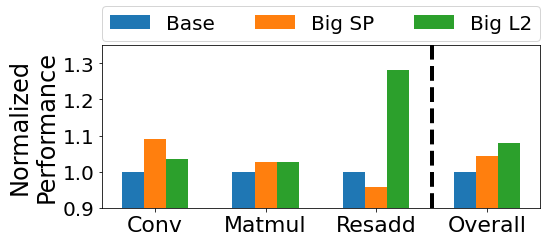
\includegraphics[width=\linewidth]{fig/dual-core-contention.png}
      \caption{Performance of dual-core SoCs.}
      \label{fig:dual-contention}
\end{subfigure}
    \caption{Performance of the various SoC configurations in the case study, normalized to the performance of the Base configuration.}
    \label{fig:contention}
    \vspace{-0.2in}
\end{figure*}

Real-world DNN applications, such as CNN inference, have diverse layer types which have different computational requirements and which contend for resources on an SoC in different ways. For example, ResNet50 includes convolutions, matrix multiplications, and residual additions, which all exhibit quite different computational patterns. Convolutions have high arithmetic intensity; matrix multiplications have less; and residual additions have almost no data re-use at all. Additionally, unlike the other two types of layers, residual additions benefit most if layer outputs can be stored inside the cache hierarchy for a long time, rather than being evicted by intermediate layers, before finally being consumed several layers later. These different layer characteristics suggest different ideal SoC configurations. To run with optimal performance over an entire DNN, a hardware designer must balance all these constraints.

% \begin{table}[t]
% \centering
% \begin{tabular}{ l | c | c | c | c }
% \hline
% Config Name & Cores & \makecell{Scratchpad\\(per core)} & \makecell{Accumulator\\(per core)} & \makecell{L2 Cache} \\  
% \hline
% \hline
% Base-Single & 1 & 256 KB & 256 KB & 1 MB   \\
% Base-Dual & 2 & 256 KB & 256 KB & 1 MB   \\
% BigSP-Single & 1 & 512 KB & 512 KB & 1 MB  \\
% BigSP-Dual & 2 & 512 KB & 512 KB & 1 MB  \\
% BigL2-Single & 1 & 256 KB & 256 KB & 2 MB   \\
% BigL2-Dual & 2 & 256 KB & 256 KB & 2 MB   \\ \hline
% \end{tabular}
% \caption{Resource contention SoC configurations}
% \label{tab:contention-soc-configs}
% \end{table}

% Point of this paragraph: Experimental setup

To demonstrate, we run ResNet50 inference on six different SoC configurations. These are the three different configurations described in Figure~\ref{tab:contention-soc-configs}, repeated for both single- and dual-core SoCs (as in Figure~\ref{fig:contention-soc}), where each CPU core has its own Gemmini-generated accelerator. The dual-core SoCs run two ResNet50 workloads in parallel, while the single-core SoCs run just one. The base design point has a 256 KB scratchpad, and a 256 KB accumulator per core, as well as a 1 MB shared L2 cache. The scratchpad and accumulator memories are private to the accelerators, but the L2 cache is shared by all CPUs and accelerators on the SoC. We presume that we have 1 MB of extra SRAM that we can allocate to our memory system, but we need to decide whether to allocate these SRAMs to the accelerators' private memory, or to the L2 caches.

% Point of this paragraph: As shown in Figure X, layers with higher arithmetic intensity benefit more from a bigger scratchpad. Memory-bound layers, like resadds, are unaffected in the single-core case

As shown in Figures~\ref{fig:single-contention} and~\ref{fig:dual-contention}, convolutional layers benefit from a larger, explicitly managed scratchpad, due to their very high arithmetic intensity. Convolutional kernels exhibit a 10\% speedup with one core, and an 8\% speedup in the dual-core case, when the scratchpad and accumulator memory is doubled by the addition of our 1 MB worth of SRAMs. The matmul layers, on the other hand, achieve only a 1\% and 3\% speedup when the scratchpad is enlarged in the single-core and dual-core cases respectively, due to their lower arithmetic intensity. Residual additions, which have virtually no data re-use and are memory-bound operations, exhibit no speedup when increasing the scratchpad memory size. Instead, they exhibit a minor 1\%-4\% slowdown, due to increased cache thrashing. In the single-core case, the increased convolutional and matrix multiplication performance is enough to make the design point with increased scratchpad memory, rather than increased L2 memory, the most performant design point.

% Point of this paragraph: However, in the dual core case, residual addition layers benefit very much from higher cache sizes

However, Figure~\ref{fig:dual-contention} shows that when we run dual-process applications that compete for the same shared L2 cache, allocating the extra 1~MB of memory to the shared L2 cache improves overall performance more than adding that memory to the accelerators' scratchpad and accumulator memories. Increasing the scratchpad size still improves convolutional performance more than increasing the L2 size, but this improvement in performance is more than negated by the 22\% speedup of residual additions that the dual-core BigL2 design point enjoys. This is because each core's residual addition evicts the input layer that the other one is expecting from the shared L2 cache, increasing the latency of memory-bound residual addition layers. The dual-core BigL2 configuration, which increases the shared cache sizes, alleviates this contention, reducing the L2 miss rate by 7.1\% over the full ResNet50 run, and increasing overall performance by 8.0\%. The BigSP configuration, on the other hand, improves overall performance by only 4.2\% in the dual-core case.

% Point of this paragraph: This demonstrates that memory partitioning schemes must be co-designed with the application in order to achieve maximum performance.

With Gemmini, we have demonstrated how the memory partitioning strategy, a key component of system-level design, can be decided based upon application characteristics, such as the composition of layer types and the number of simultaneous running processes.

%%%%%%% OLDER VERSION

% We demonstrate an example of the benefits of Gemmini's system integration by studying a system-level design decision: memory partitioning.
% Recent work~\cite{kelp} observed how host memory bandwidth contention challenges affect cloud-based machine learning accelerators (specifically, the Google TPU) in which the CPU is shared by multiple applications. In this case, the host CPU memory bandwidth is a resource under contention, since multiple CPU applications require access to memory, as well as the application running on the accelerator.

% We use Gemmini to study whether different memory partitioning design choices can impact similar resource-contention scenarios in tightly integrated edge devices. The SoC architecture under evaluation is a dual-core application processor, in which each core has a dedicated Gemmini accelerator tightly integrated with it. Therefore, the system has a total of two host processors and two Gemmini accelerators. In this SoC architecture, a shared last-level cache (L2) is shared by both the host CPUs and the accelerators, as shown in Figure~\ref{fig:contention-soc}.

%\begin{figure}
%    \centering
%    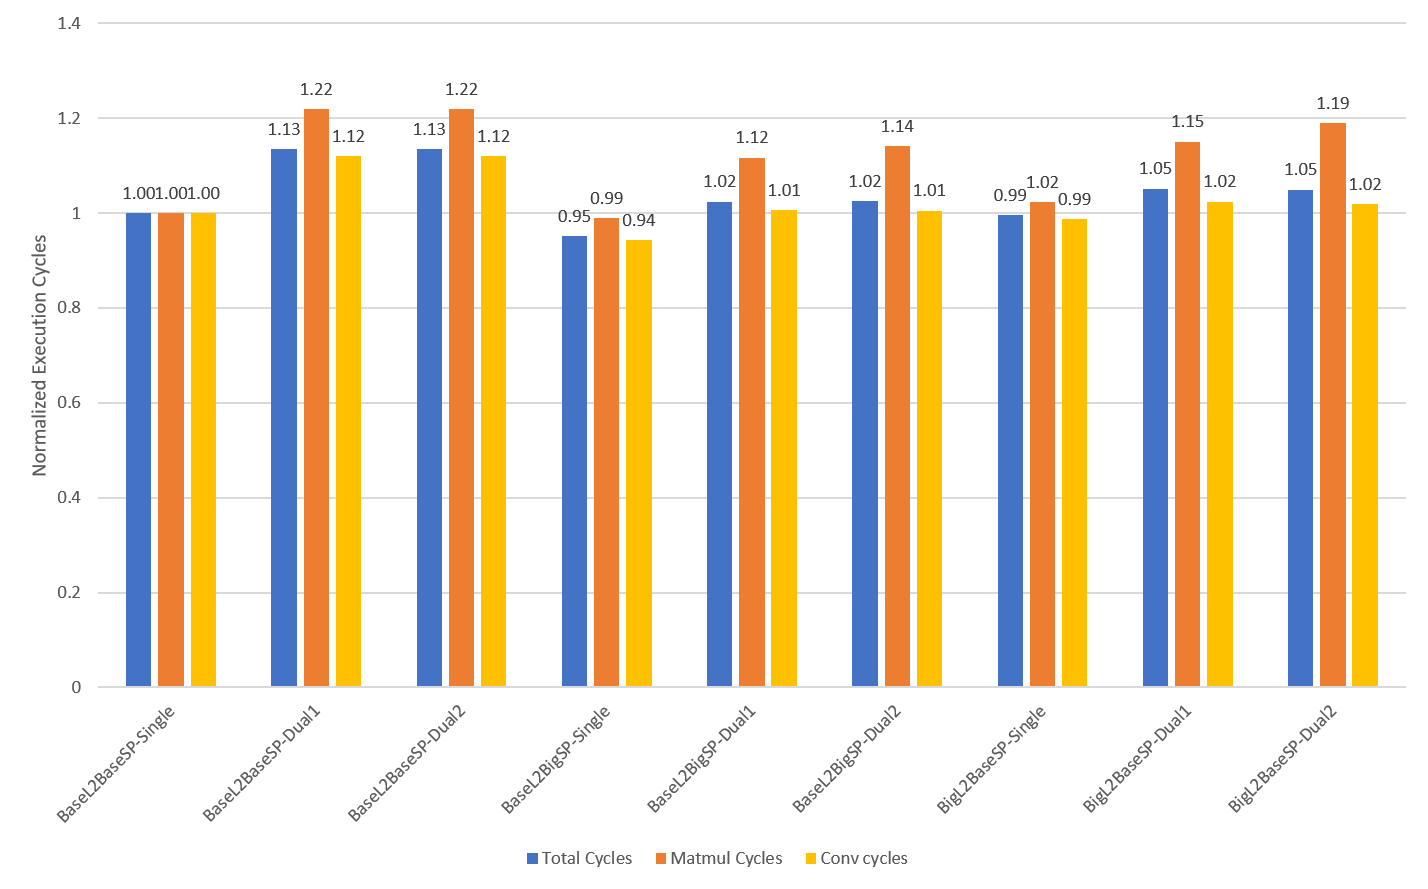
\includegraphics[width=1\linewidth]{fig/contention-normalized-perf.png}
%    \caption{Normalized execution cycles of the three SoC configurations in the last-level cache resource contention case study. For each of the three SoC configurations, the normalized execution cycles are presented for each of the ResNet-50 inference application, on each core. The execution cycles are normalized to the single-core execution of the base configuration.}
%    \label{fig:contention-cycles}
%\end{figure}


% When both application cores and Gemmini accelerators are running workloads concurrently, we would expect contention over the shared L2 to impact the execution time of each workload, compared to running the same workload on a single core individually. 
%We would also expect this phenomenon to occur when running applications which utilize the Gemmini accelerators, since their memory backend is also connected to the shared L2.

% We confirm the L2 contention expectation by measuring the performance of a ResNet50 inference application on a single core using Gemmini, and measuring the performance of two cores each executing a separate ResNet50 inference application using separate Gemmini-generated accelerators.
% The contention over the L2 resource results in a 13\% slowdown in the execution cycles of each ResNet-50 inference application over running only a single core (Figure~\ref{fig:contention} (b)), and even slightly more when examining just the cycles which utilize the accelerator.

% We explore methods to mitigate the performance impact of this resource contention by adding additional memory resources to the system. 
% The allocation and partitioning of the additional memory exposes a tradeoff between the benefits of private memories and shared memories.
% While a larger L2 should provide a benefit to all components of the target application (both those which utilize the accelerator, and those that run only on the host CPU and do not use the accelerator), greater re-use within a larger scratchpad may alleviate some of the load of L2 requests which generate the resource contention. Additionally, the benefits of a manually managed scratchpad are only as effective as the software which manages it, in contrast to a locality based cache which may provide benefits for a wider range of software implementations. 

% We study six SoC configurations, as listed in Table \ref{tab:contention-soc-configs}. As the results in Figure \ref{fig:contention} (b) illustrate, the preferred partitioning of additional memory is quite nuanced and depends on the mixture of operations within the DNN. While matrix multiplication and convolution layers benefit from re-use within the private scratchpads, residual-addition layers do not benefit from this re-use and therefore rely on L2 locality and bandwidth. Hence, increasing the size of the L2 cache improves the performance of the residual addition components while increasing the size of the private scratchpads improves the performance of convolution and matrix multiplication layers. In the single-core case, the benefits of the increased scratchpad size for convolution and matrix multiplication layers out-weighs the negligible benefits of a larger L2 on the residual additional layers, resulting in an overall improvement of XX\% compared to the baseline. However, in the dual-core case, the residual additional layers contend for L2 resources, resulting in better performance improvement in the SoC configuration with the larger L2 as opposed to the larger private scratchpads, since there is less contention between the two cores over L2 resources during the residual-addition layers.   

% We further validate this observation by characterizing the behavior of the L2 cache shared memory. Figure \ref{fig:contention} (a) illustrates the temporal behavior of the L2 cache through the cumulative number of L2 misses. As expected, the total number of L2 misses is smallest with the largest L2 cache. Similarly, the addition of a larger scratchpad also reduces the number of L2 misses (although not as much as the larger L2) thanks to a higher degree of data re-use within the scratchpads. However, we observe that while the big L2 configuration results in XX\% reduction in L2 misses compared to the baseline for the single core case, the big L2 configuration has a xx\% reduction in misses compared to the baseline in the dual-core case.
% This observation support the hypothesis of increased contention for residual layers in the dual-core case compared to the single-core case.


%\section{Case Study: Accessibility and Modifications}

%The design space expressed by Gemmini's parameters covers a diverse range of architectures, from TPU-like square systolic arrays, to NVDLA-like one-dimensional arrays of dot-product accumulators. These different designs all fundamentally perform matrix multiplications, but with different submatrix shapes, latencies, power consumptions, and critical path lengths.

%Gemmini's default configuration produces a 16-by-16 systolic array which multiplies two 16-by-16 matrices together to produce a 16-by-16 result. However, by reshaping the systolic array into a 4-by-64 array, and removing all pipeline registers between the PEs, we can produce a weight-stationary NVDLA-like design, as shown in Figure~\ref{}.

%This configuration, which we term \textit{NVDLA-like}, takes four cycles to be preloaded with a 4-by-64 set of weights. Afterwards, it receives a steady stream of data, 4 elements per cycle, from the left of the array, to perform 64 dot-products (each on two four-element vectors) every cycle.

%We find that the NVDLA-like design experiences X\% better performance on ResNet50, due to the shorter latency and faster preloading time. Total utilization of PEs increases from X\% to X\%, as seen in Figure~\ref{}.

%However, we also find that the increased critical path lengths, due to the removal of pipeline registers, reduces the maximum synthesizable frequency from 1 GHz to X MHz, on the Intel 22FL process.

%Based on one's power, performance, and physical design requirements, they may choose differently how to configure their accelerator. Gemmini enables these design-space explorations, and our push-button flow makes it simple to quantify the associated trade-offs.

% Architects have complete control over which components they want to actually generate. Our libraries are written to be flexible, so that if an accelerator engine is missing, we can fall back on slower implementations that are available.
% Students were able to take advantage of this in EE 290-2 class. Many students, including ones with very little hardware experience (and no Chisel experience) were able to design new features as well.

% Peking TVM people also took advantage of this CARRV. \textcolor{red}{Did they really? How?}

% \textcolor{red}{Should we also talk about software configurability here?}

% Notes:
% \begin{itemize}
%     \item Can choose whether or not to include pooling engine, etc.
%     \item Students showed that it's quite possible to add new operator support
%     \item Gemmini frontend: coarse-grained vs fine-grained software support
% \end{itemize}

% How do we add new instructions in Gemmini?
% \begin{enumerate}
%     \item Add new ISA instruction to gemmini.h (only 3 lines change)
%     \item Add RTL functional unit
% \end{enumerate}

% \subsection{Programming Interface Granularity}
% \label{fine-grained_inst}

%We support both fine-grained and coarse-grained instructions, with our customizable frontends. This gives us the best of both worlds over something like NVDLA and \textcolor{red}{[insert low-level accelerator here]}.
%This allowed us to rapidly come up with convolutions with and without \texttt{im2col}, both in hardware and in software.

%We support both fine-grained and coarse-grained instructions, with our customizable frontends. \textcolor{red}{(We haven't mentioned customizable frontends yet in the paper. Should we?)}

% \hl{
% We investigate how Gemmini's multi-level programming interface, described in Section~\mbox{\ref{software}}, allows programmers to write routines that can take advantage of new or uncommon kernels in which high-level programming interfaces may not support. While Gemmini is designed primarily for DNNs, we demonstrate how its flexible programming interface, which provides both high- and low-level control options, enables Gemmini to accelerate non-DNN kernels. In particular, we evaluated the ``sampled dense-dense matrix product'' (SDDMM) kernel, a known bottleneck of factor model algorithms~\mbox{\cite{Canny2013BigDA}}.
% }

% \hl{
% The SDDMM kernel can be expressed with the equation, $C = S\circ(AB)$.
% In this kernel, a sparse matrix $S$ samples out of the result of a dense matrix multiplication, \textit{i.e.}, $AB$.
% In particular, the sampling matrix $S$ is extremely sparse, whereas $A$ and $B$ are dense matrices multiplied with a standard dense matrix multiplication.
% $\circ$ is an element-wise Hadamard operator.
% The output matrix $C$ only has valid data where the sampling matrix S has non-zero elements. % , as shown in Figure~\ref{fig:sddmm-basic}.
% }

%For new workload that was not previously exposed Fine-grained instructions have advantages in flexibility that users can invoke matrix multiplication wherever they want. The representative example that leverages this benefit would be sparsity computation. With fine-grained instruction, users can selectively invoke data loading and computation where there is non-zero data. 

%Data movement instructions in fine granularity operate with granularity of mesh dimension (DIM) specified by RTL configuration. Local scratchpad, accumulator addresses and memory addresses to store and load data are specified for each instruction.
%Computation commands also follow mesh granularity (DIMxDIM). However, coarse-grained instructions pack small granularity instructions into one big instruction, which indicates ability to precisely control addresses of each command is lost.

% \begin{figure}[t]
%     \centering
%     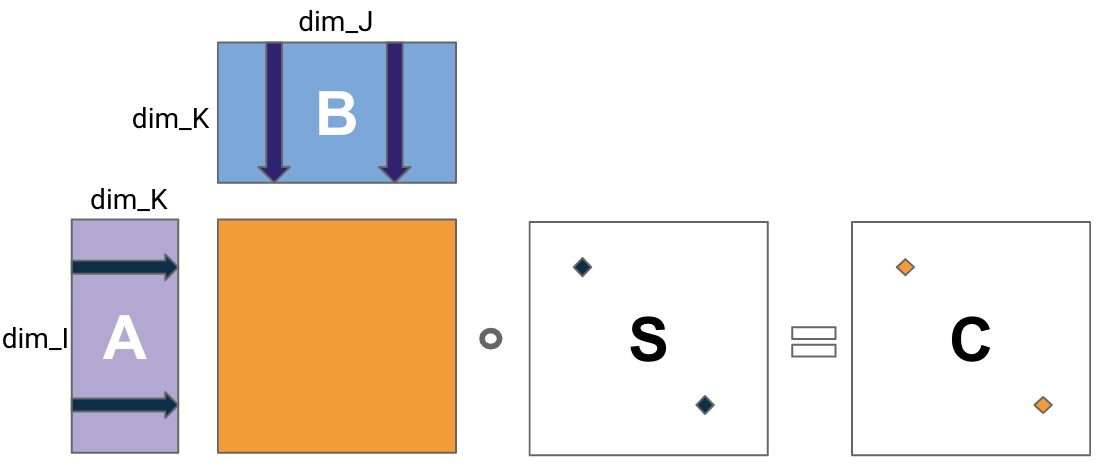
\includegraphics[width=0.9\linewidth]{fig/SDDMM-basic.png}
%     \caption{Visualization of an SDDMM operation. The arrows mark rows and columns of $A$ and $B$ which correspond to non-zero elements of the sampling matrix $S$.}
%     \label{fig:sddmm-basic}
% \vspace{-0.3cm}
% \end{figure}

% \hl{
% An efficient implementation of the algorithm would therefore skip regions in which the values of the sampling matrix $S$ are zero.
% %By identifying the non-zero elements of matrix $S$, we can compute only those rows and columns of A and B that correspond to those non-zero elements.
% By detecting the indices of these nonzero elements of $S$, programmers can use Gemmini's low-level programming interface to skip both the data movement and computation of the zero regions, while only invoking matrix multiplication at the non-zero regions. With Gemmini's low-level programming interface, programmers can load and operate on arbitrarily small pieces of data.
% By contrast, many higher-level programming interfaces expect large matrices as inputs, and are optimized for long-latency, high-throughput operations, which would not be suitable in such a sparse scenario.
% % Since Gemmini's smallest predication granularity is the spatial array dimension, an additional small bitmask can be applied to the computed results when they are moved back from the accelerator to the host processor.
% }

% \hl{
% We evaluate this approach using sparse sampling matrices from the Large Network Collection~\cite{snapnets} and Network Repository~\cite{networkrepo}. To explore a range of sampling density patterns, we evaluate two matrices with a low-density factor of less than 0.01\%, as well as a pair of sampling matrices with higher density factors of 2.5\% and 1.8\%. %Table~\ref{tab:sddmm_dataset} lists the sampling matrices dataset.
% The matrices are stored in Compressed Sparse Row (CSR) format~\cite{SpMV_CSR}.
% %Using the CSR row index pointer array, it is easy to identify which rows hold nonzero data. The exact nonzero data coordinate (i,j) can be determined by using the column indices array.
% For every non-zero element of $S$, we invoke Gemmini's fine-grained, low-level API to move the data and perform matrix multiplication.
% }

% \begin{table}[h!]
% \begin{center}
% \begin{tabular}{ p{2.1cm}||r |r|r|r  }
%  \hline
%  Dataset& Rows & Columns & \makecell{Non-zero\\Elements} & Density ($\%$)\\
%  \hline\hline
%  email-Eu-core & 1,005 & 1,005 & 25,571 &2.53\\
%  socfb-Amherst41 &2,235 & 2,235 & 90,954 & 1.82\\
%  scc\_rt\_lolgop & 9,742 & 9,742 & 9,020& 0.0095\\
%  scc\_rt\_gmanews&8,330&8,330&2,156&0.0031\\
%  \hline
% \end{tabular}
% \end{center}
% \caption{Dataset for sparse sampling matrix $S$.}
% \label{tab:sddmm_dataset}
% \end{table}

% Therefore, most rows and columns of A and B matrices would have to move in and compute, which end up only adding indirection overhead without effectively skipping anything.

% \hl{
% %The density and sparsity patterns of the sampling matrix S impact the optimal dimensions of the Gemmini spatial array.
% %We notice that the sparsity-pattern in the sampling matrices that were evaluated was such that a very fine-grained spatial array was required in order to identify zero-blocks at a DIM$\times$DIM granularity. Therefore, the kernel was evaluated with a Gemmini spatial array dimension of 4$\times$4.
% Figure~\mbox{\ref{fig:sddmm-perf}} shows performance comparisons of the SDDMM kernels with Gemmini's mid-level and low-level APIs across different datasets running on a Gemmini-generated accelerator with a 4$\times$4 spatial array. The results are normalized to the CPU performance running the same dataset.
% The mid-level API provides only an optimized dense matrix multiplication, while the low-level APIs give programmers the full control to skip unnecessary computation and data movement.
% Compared to the CPU baseline, we notice although the accelerator outperforms the CPU baseline for relatively dense datasets, CPU performs significantly better for the extremely sparse cases, especially compared to mid-level APIs.
% The reason for that is because of the non-trivial overhead of invoking accelerators and shuffling data in and out of accelerators.
% In addition, when the dataset is extremely sparse with less than $0.001\%$ density, CPU can operate directly at the scalar level for the dense region while our accelerator has to operate at the spatial-array granularity.
% }

% \hl{
% Comparing the mid- and low-level API performance, Figure~\mbox{\ref{fig:sddmm-perf}} shows that the low-level API outperforms the mid-level API by 306$\times$ for the extremely sparse matrices and 1.8$\times$ for the relatively dense ones. % (the high-level ONNX API was not evaluated since SDDMM is not an ONNX DNN operator.
% %The sampling matrices with the lowest-density factors exhibit a 306$\times$ performance improvement compared to the mid-level programming API, while sampling matrices with the higher density factors (density $>$ 1.5\%) only show 1.8$\times$ performance improvement.
% This is because the higher-density sampling matrices still have to absorb the overhead of the CSR data-structure traversal, but are not able to leverage the fine-granularity of the low-level API to skip zero regions due to the higher density.
% The results demonstrate that by using Gemmini's low-level programming interface, we are able to skip data movement and computation efficiently by using of fine-grained, small-granularity instructions which we could not have done efficiently if only high-level APIs were available.
% }

%\section{related work}
Systolic architectures first came into prominence in the early 1980s~\cite{why-systolic, kung1979systolic}, and since then, many systolic accelerators have been developed.
There has also been much work on algorithms which can design new systolic arrays methodologically, rather than through ad-hoc intuition~\cite{algoinfo}.

Early systolic arrays were used to compute convolutions~\cite{kungconv}, solutions to triangular linear systems~\cite{why-systolic}, matrix multiplications, and more. Systolic architectures enable modular and extensible designs, use local neighbor-to-neighbor message passing, and contain easy-to-floorplan regular structures.
%especially by discouraging difficult-to-route global signals.

Systolic architectures have recently regained popularity, since the convolution and matrix multiplication kernels common in machine learning and deep learning application are highly susceptible to multi-dimensional acceleration using systolic arrays.  

% Industry DNN accelerators:
Commercially deployed ASIC implementations of NN accelerators include the Google TPU \cite{tpu} for cloud workloads, as well as edge inference implementations by Samsung \cite{samsung}, Nvidia \cite{nvidia}, Apple \cite{apple}, and Tesla \cite{bannon2019accelerated, bannon2019systems}. In particular, a detailed description of the original TPU implementation includes a $256\times256$ matrix multiplication unit implemented using a reduced-precision systolic MAC array with a weight stationary dataflow for NN inference in the cloud. Successor versions included floating-point representation, additional memory, and improved utilization for both training and inference \cite{tpu2_3}.

%To target ML workloads in the cloud, Google designed the custom TPUv1 ASIC~\cite{tpu}, which uses a weight-stationary (WS) 256x256 systolic MAC array at its core to accelerate GEMM. The successor TPUv2 and TPUv3~\cite{tpu2_3} ASICs utilized a similar systolic array, added more memory, and used multiple arrays to improve utilization. The cloud TPUs were designed to accelerate both training and inference, while another ASIC, the edge-TPU, was optimized for energy efficient inference only for edge devices. Other industry players, including Samsung~\cite{samsung}, Apple, Qualcomm, and Tesla have designed inference accelerators utilizing systolic arrays. \textbf{TODO: add citations, or remove this sentence}.

Prior work has demonstrated the integration of an open-source commercial DNN accelerator (NVDLA) with the Rocket Chip ecosystem and the FireSim platform \cite{farzad2019rocketnvdla}. The accelerator in this work was integrated using the memory bus, as opposed to Gemmini which is integrated using the RoCC interface. %and enables full design-space demonstrated using Gemmini. 
Prior work ~\cite{seldridge} has also demonstrated the integration of academic NN accelerators with the Rocket Chip ecosystem using the RoCC interface, but did not use systolic architectures for that purpose.
Gemmini puts an emphasis on enabling design space exploration rather than single design-point integration.
%Eldridge et. al. proposed an NN accelerator, DANA~\cite{seldridge}, integrated as a co-processor for Rocket using the RoCC interface, however the accelerator was only capable of executing multi-layer perceptrons and not convolutions.

Academic researchers have proposed numerous systolic accelerators, especially for neural-network inference. For example, NeuFlow~\cite{neuflow} was a systolic-inspired architecture which allowed individual processing elements (PEs) to be re-configured at runtime to perform tasks such as multiply-accumulates, divisions, and non-linear activations. ShiDianNao~\cite{shidiannao}, similarly, allowed PEs to be reconfigured at runtime to perform multiply-accumulates, additions, and max poolings. 
Eyeriss~\cite{eyeriss} implemented a weight-stationary dataflow using a spatial array. Eyeriss v2~\cite{eyeriss2} improved on the original Eyeriss by demonstrating a new PE architecture that can operate on sparse CSC-encoded matrices, and a hierarchical mesh NoC capable of unicast, multicast, and broadcast data transfers to maximize reuse.
These and other systolic-inspired architectures typically permit both global and local connections between PEs and global memory, which is not strictly systolic, but often improves performance.

%Chen et. al. proposed Eyeriss\cite{eyeriss}, a convolutional layer accelerator implemented as a spatial array of PEs computing using a weight stationary dataflow. Eyeriss utilized a NoC to support multicasting weights to several PEs, and had a 2-level memory hierarchy consisting of a large buffer SRAM and PE-local input, weight, and partial sum register files. Eyeriss v2\cite{eyeriss2} demonstrated a new PE architecture that can operate on sparse CSC-encoded matrices, and a hierarchical mesh NoC capable of unicast, multicast, and broadcast data transfers to maximize reuse. While Eyeriss proposed a novel architecture, the work did not explore the full design space and evaluate how different accelerator parameterizations affect throughput and energy efficiency.

%talk about flex-flow as a multi-dataflow proposal
Several previous proposals~\cite{squeeze, lu2017flexflow, fu2017} have presented performance and energy benefits resulting from flexible data-flow options in NN accelerators. However, the benefits and impact of the dataflow structure of NN accelerators is still an active area of research, and some works~\cite{overrrated} have shown that optimal memory-hierarchies and loop-blocking strategies can have a more significant impact on energy efficiency than the choice of dataflows. 

%Talk about ISSCC/VLSI accelerators
Various energy efficient neural network accelerator proposals have also been presented in the integrated circuits community \cite{ueyoshi2018quest, lee2018unpu, bankman2018always, karnik2018cm, shin201714, yin20171, ando2017brein, kim20192, sayal201914, lee20197, yue20197}. Many of these proposals focus on exploiting sparsity and quantization features of DNNs. Furthermore, while some of these proposals address runtime-configurability, they still address only a single fabrication-capable design point, and most do not present design and elaboration time parameterization. Further, most of these accelerators are tested in isolation, often without a fully integrated software environment, hence potentially neglecting system-level effects. 

%talk about FPGA-based accelerators; just aggregate a bunch of citations and contrast them to ASIC implementation for peak energy efficiency
A host of DNN accelerators targeted for FPGA implementation have also been proposed\cite{zeng2018, wang2016, shen2018, dicecco2016, guan2017, guo2018, zhang2018, zhang2015, venieris2016, sharma2016, zhang2017, wang2017}, taking advantage of FPGA reconfigurability to implement exotic layers, specialize the hardware for a specific network, and evaluate multiple design points. However, FPGA acceleration frameworks do not necessarily translate well to ASIC implementations, and are not ideal for scenarios where energy efficiency is critical.

%talk about ISCA/MICRO/HPCA/ASPLOS Simulated accelerators
% Karu Sankaralingam (Wisconsin) - CGRAs (nowatzki2017) - SW simulated on model, but they have Chisel RTL too
Some prior works \cite{yazdani2016,song2017,srivastava2018,sharify2018,squeeze,angizi2018,min2019,nowatzki2017} use analytical or high-level model-based simulations to evaluate different parameterizations of a proposed accelerator architecture. 
%While modeling is useful to explore a design space, it is difficult to validate the model unless there is corresponding RTL and the physical implementation of the circuit. 
In contrast, Gemmini performs design space exploration on the RTL directly and uses feedback from FPGA-accelerated simulation and physical design to find optimal design points for ASIC implementation.

%Processing in Memory
% Jishen Zhao - in-memory compute for DNNs (liu2018,chi2016)
% Lide Duan - NVM crossbar arrays for DL acceleration (yan2018)
% Jing Li (Wisconsin) - ML accelerator stuff (zha2019 - Liquid Silicon)
% Yuan Xie (UCSB) - PIM with ReRAM, FPGA stuff (ji2019,chang2019)
Since the energy consumed during DNN inference and matrix multiplication is often dominated by external memory accesses, academic researchers have proposed processing in memory\cite{liu2018,chi2016,yan2018,yan2018_2,zha2019,ji2019,chang2019}. These works include the development of new SRAM circuits and the use of novel devices such as ReRAMs. Gemmini is designed and validated for CMOS implementation, and uses design space exploration to discover the ideal memory access patterns and memory hierarchy to conserve energy.

%co-design and generators
Researchers have also proposed methodological systems and algorithms to automatically generate systolic architectures directly from the algorithms they are meant to accelerate. For example, PolySA~\cite{polysa} analyzes polyhedral models to attempt to find the optimal mapping between a sequential algorithm and a set of parallel PEs. Yang et al.~\cite{overrrated} extended the Halide programming language to automatically generate C++ high-level-synthesis (HLS) implementations of systolic arrays.
%we need to have a sentence to differentiate from these

%talk about VTA (as an open-source generator/research platform with software stack
%need to mention VTA here, and talk about the fact that they focus on FPGA targets rather than ASIC
Prior work has also introduced TVM \cite{chen2018} and VTA \cite{moreau2018} as an integrated research platform for SW/HW evaluation of NN accelerators. While Gemmini and VTA hold many architectural similarities, including the use of a GEMM core, explicit memory management, and explicit instruction dependency handling, VTA has primarily targeted FPGA accelerators implementations, as opposed to Gemmini which currently targets primarily ASIC designs and has been used in the fabrication on multiple test-chips. Furthermore, Gemmini's integration with the RISC-V eco-system enables an additional level of customization in SW/HW co-design. 

%Chen et. al. proposed TVM\cite{chen2018}, an open-source DNN compiler stack capable of ingesting a compute graph, optimizing it for a particular architecture, and optionally delegating inner kernels to specialized accelerators. Moreau et. al. proposed VTA\cite{moreau2018}, a decoupled accelerator with a tensor ALU and GEMM core, and a CISC ISA with explicit memory management and instruction dependency handling. VTA integrates with TVM by using a JIT compiler to lower TVM IR at runtime, and by using TVM's tensorization intrinsic. TVM and VTA form a full stack environment for DNN acceleration, however the VTA targets an FPGA implementation, whereas Gemmini targets an optimal ASIC design.



% PC Members to Cite
% Lu Peng - Fooling AI with AI (too far from our work)
% Antonio Gonzalez - RNN accelerator (http://arco.e.ac.upc.edu/wiki/index.php?title=Publications) (not sure where to cite the RNN accelerator - E-PUR)

% \textcolor{red}{Hasan, Done by 4th of May} \\
% 2.1 systolic arrays \& Inference \\
% 2.2 back to the nineties\\
%     UCSD\\
%     Eyeriss\\
%     TPU -- all versions\\
%     Tesla GPU\\
%     Dataflows are overrated\\
%     Samsung?
%     others?



%Recent accelerators designed by architects in industry have helped to rekindle interest in systolic architectures. Google's TPUv1~\cite{tpu}, for example, is built around a weight-stationary 256-by-256 systolic array which performs matrix multiplications, as is Tesla's ``Accelerated Mathematical Engine''~\cite{tesla}.


%Systolic architectures have regained popularity as machine learning workloads have proliferated in the cloud and at the edge. Common kernels such as GEMM and 2D convolution are used extensively in modern DNNs and systolic hardware accelerators can achieve optimal energy efficiency and performance.

%Yang et al. \cite{overrrated} concluded that a systolic array's dataflow does not have a significant effect upon performance or power consumption, assuming that its memory hierarchy and loop-blocking strategy are optimal. Complementary work from Kwon et al.~\cite{squeeze} suggests that different dataflows have a different impact on different layer types, and hence multi-dataflow accelerators can provide some performance and energy benefits.
% \vspace{-0.05in}
\section{Conclusion}
% \vspace{-0.1in}
We present Gemmini, a full-stack, open-source generator of DNN accelerators that
enables systematic evaluations of DNN accelerator architectures.
Gemmini leverages a flexible architectural template to capture
different flavors of DNN accelerator architectures.
In addition, Gemmini provides a push-button, high-level software flow to
boost programmers' productivity.
Finally, Gemmini generates a full SoC that runs real-world software stacks
including operating systems, to enable system architects to evaluate
system-level impacts. 
Our evaluation shows that Gemmini-generated accelerators demonstrate high performance efficiency, and  
our case studies show how accelerator designers and system architects can
use Gemmini to co-design and evaluate system-level behavior in emerging applications.

\section{Acknowledgements}

This research was, in part, funded by the U.S. Government under the DARPA RTML program (contract FA8650-20-2-7006). The views and conclusions contained in this document are those of the authors and should not be interpreted as representing the official policies, either expressed or implied, of the U.S. Government.


%%%%%%% -- PAPER CONTENT ENDS -- %%%%%%%%

% \newpage

%%%%%%%%% -- BIB STYLE AND FILE -- %%%%%%%%
\bibliographystyle{IEEEtran}
\bibliography{ref,sophia}
%%%%%%%%%%%%%%%%%%%%%%%%%%%%%%%%%%%%

\end{document}
